\chapter{\textit{It's Our Future}: the difficulties of resisting austerity-intensified capitalist realism}
\label{ch:7}

\section{Introduction}
\label{sec: 7-intro}

In the previous chapter, I constructed a grounded theory which described how austerity-intensified capitalist realism maintains hegemony and control through justification and classification practices, which result in a discursive form of accumulation built around the production of `best practice' and innovation. These practices stabilise austerity-intensified capitalist realism through the production of `vulnerability' (described in chapters \ref{ch:2} and \ref{ch:6}). In this chapter, I outline a pilot project to design against the functioning of justification and classification practices in order to destabilise austerity-intensified capitalist realism and attempt to imagine and build coherent alternatives to it. Throughout the chapter, I detail the \emph{It's Our Future} project, a design project commissioned by The Charity to support young people to think about what they wanted for their futures, and produce a manifesto that could be used to influence policymakers to work towards these futures.

I begin the chapter by outlining a set of principles for the design of methods to work against the functioning of austerity-intensified capitalist realism in the form of justification and classification practices. I then outline the initial context of the design brief set by The Charity, and define how I responded to this brief whilst developing a set of methods that could destabilise justification and classification practices. I describe how the project's focus changed partway through due to justification practices in the form of The Charity's risk aversion and fears around reputation management. I then detail the methods used in the final \emph{It's Our Future} project, which centred on building collective imagination practices for groups of people who do not know each other. I outline the use of the methods during the project and evaluate their use, finding that though they begin to meet the challenges of imagining and building alternatives to austerity-intensified capitalist realism, they fail to fully meet the scale of the challenge, indicating the need for another round of method development in chapter \ref{ch:8}. 

\section{Designing against austerity-intensified capitalist realism}
\label{sec:7-2-methods}
So far, this thesis has explored my first two research questions, which explored the experiences and affects that capitalist realism elicited and how capitalist realism makes these experiences affects possible (or probable). In the next two chapters, I will be exploring my third research question, which asks "How can the tools and methods of design be used to respond to the challenges presented by capitalist realism?". In this section, I will outline why design methods are a suitable approach to responding to the challenges posed by austerity-intensified capitalist realism, and what a design response to austerity-intensified capitalist realism must feature in order to potentially be successful. 

As explored in chapter \ref{ch:3}, designed artifacts act as both an embodiment of knowledge and a catalyst for further knowledge creation, as both mediating objects and meaningful tools simultaneously. The design methodology I developed in that chapter drew most centrally upon participatory design, critical design, prefigurative design and speculative design, which I will briefly revisit in order to highlight their contributions to my design approach. Participatory design approaches bring a sensitivity to issues of power and participation that are integral for designing to support the experiences of care-experienced young people and the workers who support them in the context of justification practices. Critical design approaches lend a focus to the design of objects that reflect or refract something about a dominant social order in order to stimulate discussion. Prefigurative design approaches suggest that social change can be made through design processes themselves, rather than just as the outcome of a design process. Finally, speculative design acts as a development to critical design by explicitly anchoring the objects of speculative design around the construction of our current world or potential futures. I draw on each of these design traditions in my own approach against the functioning of austerity-intensified capitalist realism. 

In the previous chapter, I outlined the key features of justification and classification practices, and explored how these lead to a discursive form of accumulation which entrenched the hegemony of austerity-intensified capitalist realism. These drew on a set of experiences and affects explored in chapter \ref{ch:5}. Any successful design response to austerity-intensified capitalist realism, then, must seek to ameliorate the experiences and affects explored in chapter \ref{ch:5} whilst either operating around the mechanisms described in chapter \ref{ch:6} or disrupting how these function. To turn first to workers, then, a successful design response might:
\begin{itemize}
    \item reduce workloads or provide workers with the tools to navigate their workplaces more comfortably,
    \item support workers to either do work they are skilled at, or to gain skills at an appropriate pace, or
    \item build more trusting relationships between workers and managers, or reduce managers' use of control techniques.
\end{itemize}
A successful design response for young people perceived to be vulnerable might:
\begin{itemize}
    \item prioritise their agency and ensure they are meaningfully listened to,
    \item listen authentically and follow through on what has been heard, or
    \item ensure they receive the right support. 
\end{itemize}
In all, a successful design response to austerity-intensified capitalist realism must support both workers and young people perceived to be vulnerable to become less anxious, confused, distrustful, or powerless by changing the dynamics of the systems they are existing within. 

These design responses will have to either disrupt the functioning of justification, classification, and discursive accumulation practices, or will have to find a way to work around them. They must therefore find ways to act against:
\begin{itemize}
    \item the prioritisation of evaluation (whether by skilled or unskilled evaluators),
    \item breaking projects up into granular outcomes and outputs, which are then used to justify the organisation's practice,
    \item the stratification of support according to the (funding-linked) identities of young people, and
    \item the production of `best practice' and innovation through discursive accumulation.
\end{itemize}

Working against capitalist realism in any form must counter the notion that "capitalism [is] the only viable political and economic system\ldots{} [and] it is now impossible even to imagine a coherent alternative to it" \citep[p. 2]{fisher_capitalist_2009} and the "slow cancellation of the future" \citep[p. 5]{fisher_ghosts_2014} that results from this. As such, the aim of using the tools and methods of design to respond to the challenges posed by austerity-intensified capitalist realism must be to create anticipatory practices that destabilise the feeling of necessity posed by the futures presented out by austerity-intensified capitalist realism. Rather than participants feeling as if "the whole system is like a pressure cooker about to explode" (as one participant described in the previous chapter), or the hopelessness that results from someone saying they'll be for you and not being there for you (as Scarlett described in chapter \ref{ch:5}), these design methods must create a sense of possibility about the potential of different futures.

\section{Project context}

Whilst working with The Charity on the projects described in previous chapters, a potential new project come onto the horizon, at that point entitled \textit{FutureYoungPeopleUK}. This project was intended to be a large scale digital consultation to better understand what young people wanted for their futures at a time when The Charity had felt their wants and needs had been largely overlooked. In the year prior to this, for example, there had been repeated uproar about the United Kingdom leaving the European Union (`Brexit’). For months, there had been no significant movement on the terms of the withdrawal agreement, and when there finally was, it failed to make its way through Parliament. What followed included a Conservative Party leadership election, an illegal prorogation of Parliament, a swing towards `hard Brexit’ (unilaterally leaving the European Union without a trade deal) and, towards the end of this project, a general election was called. In all of this, there had been a great deal of frustration from young people – either from those who were too young to vote in the 2016 European Union membership referendum, or from those who felt the future of the country was being unfairly decided by those who wouldn’t have to deal with the consequences of it. As part of this, groups such as \emph{For our Futures’ Sake} and \emph{Our Future, Our Choice} were established with the backing of the People’s Vote campaign to attempt to highlight the need to consider young people’s wants and needs for the future \citep{noauthor_for_2019} \footnote{Websites for these groups no longer exist due to the ephemeral nature of this kind of activism, and as such must be cited via limited archival snapshots}.

The idea for \textit{FutureYoungPeopleUK} came against this backdrop. Alongside a decade of austerity and a lack of prioritisation of services for children and young people in government budgets for years, The Charity were keen to run an event that brought young people’s wants for the future and their inability to effectively influence official discourse around the future to prominence. The form of \emph{FutureYoungPeopleUK} changed rapidly across the two months that I was designing and developing it. In its final form, it was \emph{It’s Our Future}, a large-scale design workshop and participation event for young people to imagine and build the future, but it began as \emph{FutureYoungPeopleUK}, a digital intervention designed to connect young people about their wants for the future in a novel way. 

The Charity was part of a ‘civic leadership group’ composed of senior civil servants, CEOs of charities and other interested stakeholders who had become concerned about the lack of consideration of the experiences and needs of young people within civil society. In response to this, they commissioned YouGov to conduct a poll which was responded to by 1036 young people, exploring how they felt about the future, and what events felt might transform their lives in the next five years. The headline outcomes of this work were that most young people either felt uncertain about the future or felt negatively about it, thinking that they would be worse off than they are now (which my fieldwork also supported), and that the main things that they felt would transform their lives were having money, having a better job, getting a degree, becoming healthier, and having better mental health. This survey was being conducted across all young people,  however, and The Charity wanted to understand whether or not their service users' wants and needs were different from these. The civic leadership group agreed that it was important that they did more than synthesise the results of this survey, desiring an attempt to actively ensure that the voices of young people "shaped, developed, and articulated an agenda for action, for themselves and for the country". 

This project was being undertaken by The Charity's senior management, and throughout the project I worked with multiple members of The Charity's leadership team. This was part of my original desire to do this project - other opportunities to engage with different projects within The Charity had arisen before, but the opportunity to work this close to the decision-making power inside of the organisation was important to me, both for understanding justification practices more closely and for developing an approach to work against justification practices and austerity-intensified capitalist realism. In The Charity's regional projects, there would occasionally be an appeal to a higher authority as to why they couldn't make a change - explaining that they were powerless to the wider organisational policy. Working directly with the people who could change organisational policy seemed to me to be a sensible way to understand the range of possibilities for altering justification practices, although it came with its own issues which I detail later in the chapter.

Even at the outset, the project was attempting discursive accumulation. Although the project's aims (ensuring that young people perceived to be vulnerable are put at the heart of policymaking at a time when they were being further disenfranchised) were commendable, The Charity was attempting to position themselves as a leader and innovator within this practice. Of particular note here is my closest contact during this project - Martin, the Director of the Central Services Innovation Fund (who was Michael's manager, one of the people that had been placing pressure on him throughout the Building Bridges project). At the conclusion of the project, Martin would be leaving the organisation, and multiple people from within The Charity noted that this was intended to be something of a "victory lap" for him as he left the organisation, to celebrate the work of the first 3 years of the Central Services Innovation Fund. I was aware this meant that attempts at discursive accumulation and justification practices would occur throughout the project, and would be a significant constraint to design around. 

\section{The initial project: developing movement-building methods through social media}
Martin and his team's original idea for the project centred on a two week digital conversation that I would design, facilitate and deliver, the output of which would be used to feed into the design and delivery of a launch event for a wider programme of civic engagement.  In the first instance, then, my designs responded to this brief: a two-week digital conversation that could feed into the design of an in-person launch event. Because of the quick turnaround of the project, I worked on the project with a team of volunteers from within my university research group. This team was composed of the following people (with their project roles in brackets):
\begin{itemize}
    \item Daniel Parry (designer and digital content creator, facilitator)
    \item Emily Barker (communications and movement specialist, facilitator)
    \item Sean Peacock (researcher of youth participation, facilitator)
    \item Mohaan Biswas (junior researcher, facilitator)
    \item Velvet Spors (researcher of games, facilitator)
    \item Sara Armouch (facilitator)
    \item Daniel Lambton-Howard (researcher of social media and games)
    \item Adam Parnaby (researcher of inequality and games)
    \item Ian Johnson (researcher of democracy and citizenship)
    \item Rebecca Nicholson (researcher of education and creativity)
\end{itemize}
The initial plan was for this "digital conversation" to begin with a set of simple asks on social media and to recruit participants from their responses to a smaller group on a different platform. We would then run activities with this smaller group in order to support them to build and grow a movement of like-minded young people. As such, my design process centered around identifying ways to developing effective movement-building methods in a short period of time and infrastructuring young people's participation so that a simple initial engagement could lead to a young person becoming more deeply involved and changing how they think about the future.

\subsection{Developing quick, effective movement-building methods}
Although I recognised that the project and event were likely to contribute towards discursive accumulation, I hoped that some of the worst of this could be avoided if I was able to gather together a group of young people who were interested in making social change and supported them to develop the skills (and resources) needed to make social change. In doing so, I hoped that the authentic change created through this would offset The Charity's attempts at discursive accumulation. As such, I recognised that myself and the project team needed to quickly understand some of the methods and techniques used by activist movements and protest groups throughout history, and the theory that had been built around effective movement-building. In the historical review, we began to research the techniques and tactics from recent social movements such as Occupy, the Arab Spring, and impactful union strikes throughout history, but there was not enough time to unpack the movements from the nuanced contexts that they arose from. Instead, we turned towards practice-based theories of movement-building. Three useful concepts emerged during this process that we used as anchors throughout the rest of the project – counterpower, emergent strategy, and research justice. We threaded these three concepts throughout the project and they became core to the project's intended outcomes. 

I was drawn to Tim Gee’s work on counterpower \citep{gee_counterpower:_2011} as it complemented my existing analysis of the hegemony of austerity-intensified capitalist realism presented in chapter \ref{ch:2}.  Gee defines counterpower in three ways, centered on ideas, economics, and physical power. Idea counterpower revolves around the refutation of existing ideas and identification of new channels of communication. Economic counterpower is an expression of power through the economy, i.e. through strikes, boycotts and changes in consumption habits. Finally, physical counterpower is the movement of people to disrupt systems of power - through either violent or nonviolent means \citep[p. 13]{gee_counterpower:_2011}. No matter which conception of counterpower is used, in the context of this thesis it can be thought of as building an alternative centre of power to the hegemony of capitalist realism. Building counterpower is building the capacity of individuals and collectives to create movements and centres of power that are not located within capital, and which can act as a counter hegemony \citep[p. 19]{gee_counterpower:_2011}. 

Gee identifies four key stages to building counterpower – consciousness, co-ordination, confrontation, and consolidation \citep[p. 130]{gee_counterpower:_2011}. Consciousness is the stage of realising that there is a problem and creating the conditions for building counterpower. This is broadly consistent with the approach of critical pedagogy explored in chapter \ref{ch:3}, in which the goal is to reach critical conscioussness,  a state whereby people are able to relate problems to their structural causes. Co-ordination is the stage of building counterpower through a movement to address that problem. Confrontation is the moment of confronting those with traditional power, challenging their power with the movement’s own counterpower. Finally, consolidation is about maintaining counterpower after it has been used to confront traditional power, continuing to hold power and ensuring that turns into material change. These four stages became anchors for guiding the design of the project in both its initial "digital conversation" form and its later workshop/card game format. We referred to these as mechanisms for articulating problems, building power, confronting those with traditional power, and maintaining power. These are explored in more depth in section \ref{sec:7-5-final}. 

The work of adrienne maree brown taught us a number of foundational concepts around movement-building work that guided the methods we developed to build counterpower within the workshop. Her concept of emergent strategy was initially developed as an attempt to describe the kinds of adaptive and relational leadership that feature in the fiction of Octavia E. Butler - particularly the characters within her \emph{Earthseed} series, who are attempting to build new worlds in the shell of an old one. It then developed beyond that, to encompass "plans of action, personal practices and collective organizing tools that account for constant change" \citep[p. 23]{brown_emergent_2017}, "strategies for organizers building movements for justice and liberation that leverage... simple interactions to create complex patterns", and "how we intentionally change in ways that grow our capacity to embody the just and liberated worlds we long for" \citep[p. 24]{brown_emergent_2017}. Emergent strategy has six core elements. It is:
\begin{itemize}
    \item fractal (how we are at the small scale is how we are at larger scales),
    \item intentionally adaptive (changing whilst staying in touch with our broader visions),
    \item interdependent and decentralised (building trust, vulnerability, and deeper connection),
    \item non-linear and iterative (change isn't linear, and requires repetition),
    \item resilient (by using the tools of transformative justice for recovery and repair), and
    \item generative (by creating more possibilities). \cite[p. 50]{brown_emergent_2017}
\end{itemize}
We drew on the ideas of emergent strategy throughout the design process, and constantly referred back to it to help determine if our methods were meeting their aims. For example, the "fractal" element of emergent strategy helped us to realise that even the smallest interactions would be integral to designing a process to build a movement. As a result, we focused in on developing methods to build trust between participants early into the process, so that they could build strong relationships which might support them throughout the social change they wish to make. We also realised we would have to create mechanisms to decenter individual leadership and build in opportunities for decentralised leadership and collective decision-making. Overall, emergent strategy helped us to get closer to understanding what states of being we might be trying to move people towards throughout the overall project, and how we might support them on that journey.

As explored in chapter \ref{ch:3}, research justice is a framework for conducting research that advocates for a research praxis centered on liberation and justice. It values the situated sense-making of communities, supporting them to make their own knowledges, to de-center pre-existing ideas of what is considered `legitimate' knowledge, and to support greater community control over the whole knowledge production lifecycle. As this was a project that was already drawing heavily on ideas of building power within communities of lived experience, it felt important to prioritise ideas of research justice within it. Research justice drew our attention towards creating mechanisms for our participants in the project to create their own knowledge and analysis of the world as they experience it, and to de-center the experiences and power of workers and "civic leaders". In practice, this meant identifying ways to preserve the integrity of what young people were saying and doing throughout the project, and attempting to hold back some of The Charity's attempts to co-opt the project. In doing so, we hoped we might limit some of the power of discursive accumulation by using our own power and privilege as researchers to create space for young people to follow the approach they wanted to.

At this stage, we had a better understanding of the methodological requirements of the project. This project would explore designing against the functioning of austerity-intensified capitalist realism by focusing on young people perceived to be vulnerable. It would prioritise their agency and ensure they receive the right support by creating the circumstances for them to articulate their issues with the world as they experience it, identify alternatives, and work towards these. This could disrupt The Charity's tendency towards justification, classification, and discursive accumulation by supporting young people to act outside of the constraints of The Charity, in ways that couldn't be easily evaluated by them, and which could not be broken up into granular outcomes and outputs. The project would be an attempt to enhance the counterpower of young people perceived to be vulnerable, as they went through the stages of articulating problems, building power, confronting those with traditional power, and maintaining power. Where possible, young people would be supported to develop skills, rather than have a member of the existing team do something for them, creating space for their own situated sense-making. Finally, we would draw upon the elements of emergent strategy to construct a process throughout the digital conversation that would support the group to imagine different potential futures, build trust between themselves, and identify pathways towards making these changes.  

\subsection{Infrastructuring participation through social media}

Outside of indicating that they wanted a "digital conversation" to take place, The Charity did not give us a particular steer on what form they wanted this to take. We initially considered running the project on a custom-designed platform, but we felt that for ease of use, timing, and accessibility, it would make the most sense to initially draw on social media platforms for this digital conversation. When considering which platform(s) to use,  we conducted a rapid review of trends within social media engagement for charities and other groups that work with young people. I also reflected on this from the perspective of my prior engagement with The Charity, including a participatory user experience research project I conducted with The Charity which does not feature within this thesis (on young people and worker's uses of technology). I divided the potential platforms into four categories: text-based (posts), text-based (messages), image-based, and video-based.  The platforms are shown within these categories in table \ref{table:iof-social-media} \footnote{Many of these social media platforms now employ features from other platforms (such as Instagram \textit{Reels} or YouTube \textit{Shorts} which are clones of TikTok, or the \textit{Stories} feature which originated on Snapchat but now exists on Facebook, Instagram, WhatsApp, and briefly existed on Twitter.)}.

\begin{table}[hbt!]
\begin{tabular}{lllll}
\caption{A grouping of different social media platforms (as they existed in 2019) by their primary functions. These were the platforms considered for use within the project.}
\label{table:iof-social-media}
\textbf{Text-based (posts)} & \textbf{Text-based (messages)} & \textbf{Image-based} & \textbf{Video-based} &  \\
Twitter                     & WhatsApp                       & Instagram            & YouTube              &  \\
Facebook                    & Facebook Messenger             & Snapchat             & TikTok               &  \\
                            & Discord                        &                      & Twitch               &
\end{tabular}
\end{table}
At this stage, I eliminated several platforms, both for lack of relevance to the target audience and for technological limitations. Informed by the aforementioned project around technology usage, we disregarded Facebook and Facebook Messenger for their relative lack of youth users, and disregarded Snapchat because young people had previously described it as "unprofessional" for an organisation to use it (despite its large youth userbase). Though Twitter also has a low youth userbase, we decided to include it because it is the primary social media of many charities and so we felt it would be useful for raising the profile of the engagement to other charities. We disregarded Twitch at this stage, as although it has a large amount of young users, only a very small percentage of users have high viewerships, with the majority of users on the platform being viewed by only one or two people. In particular, frequently-visited channels on Twitch tend to have built their audiences from multiple hours-long streams at a time, something we would have been unable to do due to the project's time constraints. Finally, we eliminated WhatsApp from our list of potential platforms as we wanted to potentially automate aspects of the structure of the engagement and at the time WhatsApp’s API\footnote{An Application Programming Interface (API) is the means by which one piece of software can programmatically communicate with another. In this, the WhatsApp API would have allowed us to programmatically send messages via WhatsApp.} was still in beta testing. 

This left us with five candidate platforms – Twitter, Discord, Instagram, YouTube, and TikTok. Rather than choosing to focus on just one of these, at this stage we decided to develop a strategy for infrastructuring young people's participation across all five of these platforms. At this stage, our plan was to design and develop prompts for the engagement and automate posting these across each social media platform through the use of multiple bots, which would deliver the content across each day of the engagement. We decided  that our central social media platforms for the engagement would be Instagram, Twitter and Discord, and that YouTube and TikTok could act as potential amplifiers for the engagement if we could enlist the support of some prominent YouTubers and TikTok accounts. The Charity were keen to use a snowballing recruitment strategy, whereby those that became involved with the project would encourage others that they knew to become involved, either by being visible through public interactions or through directly encouraging their friends to become involved. As such, we decided to make this a two-phase engagement. In the first phase, anyone would be able to respond to public Instagram or Twitter posts, and our follow-up engagement would help our participants to move closer to critical consciousness by asking questions that helped them to link their lived experiences to structural problems. After follow-up engagement, we would invite them to join a private organising group hosted on Discord. This organising group would be able to decide on the content to be put out onto social media for further recruitment, and would work towards the development of a manifesto of young people's ideas for the changes that would support them to live better lives. 

We aimed to start the project with the simplest possible touchpoint - responding to a single question. Our central idea was that asking questions about one’s own lived experience provides a clear and simple starting point. We set about trying to find the simplest possible question that asked what participants wanted for the future but that was grounded in their lived experiences. Initially, we began with:
\begin{quote}
What changes would you make to the country now so that you can live your best life in 3 years?
\end{quote}

We attempted to build on this, in order to draw upon the results of the YouGov survey commissioned by The Charity, but felt that this risked confusing participants by complicating the initial point of interaction. We refined our initial question further, and settled on the prompt:

\begin{quote}
Make something – whether a song, poem, drawing, video, etc. – about how you see your future.
\end{quote}

At this stage, we had a sense of the initial outline for the project. This would be a project which focused on building a movement of young people by drawing on ideas of counterpower, emergent strategy and research justice. We would recruit participants through responses to a simple ask on Twitter or Instagram, and then we would engage people to more deeply think about their initial responses (either manually or with the support of simple bots). On the basis of this engagement, we would invite people to a Discord server, where they would be able to get to know other people within the project and we would run activities for them which helped them to imagine a different, better future for themselves and identify changes that could happen at a national level that could support them moving towards these futures. This would then lead towards the creation of a manifesto that would be presented at an in-person event. Due to the changes that had to be made to the project, many of these ideas are under-conceptualised, and would have required significant refinement before moving forward, in order to ensure that the project both worked well and successfully kept participants safe. They are presented in here in this unrefined form as a few weeks before the project was due to go live, The Charity still could not agree on a way of moving forward with the project. 

\subsection{Navigating justification practices and performativity}
The Charity approached my research group because of its reputation for high-profile digital innovation projects with other charities and public sector organisations, such as the NINEtoFIVE project, the WhatFutures project, and the TalkFutures project \citep{lambton-howard_whatfutures:_2019, rainey_talkfutures_2020, abdulgalimov_designing_2020}. As explored in the previous chapter, whilst innovation practice appears to be about embracing change and novelty, it tends to reproduce the existing social order. Despite The Charity's desire for a digital innovation project that they could extract discursive value from, throughout the engagement process they repeatedly showed that they were ill-prepared to support the project organisationally or technologically. They created frequent bureaucratic and procedural issues. Just a week after the project began, The Charity asked us to visit their head offices in London to pitch our vision for the project (excerpts from the slides can be seen in figure \ref{fig:iof-pitch}). We prepared a pitch deck that reflected the project as I have presented it so far - a two-phase `digital conversation', conducted across multiple social media platforms, that would slowly filter into a core organising group that would be on Discord. Between the two phases, we would do follow-up engagement with participants in order to help them develop their ideas and proposals for the future and help move them closer to critical consciousness around the issues that they saw as key to a future. Although they broadly supported the approach, when we presented this to The Charity they had a number of concerns around safeguarding. 

\begin{figure}
    \centering
    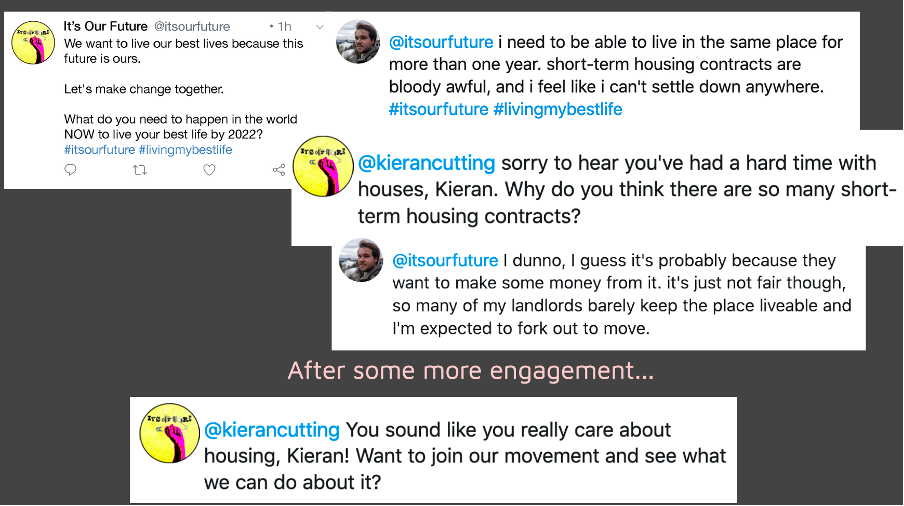
\includegraphics{Images/7/iof-1.png}
    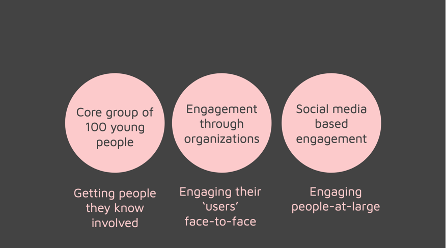
\includegraphics{Images/7/iof-2.png}
    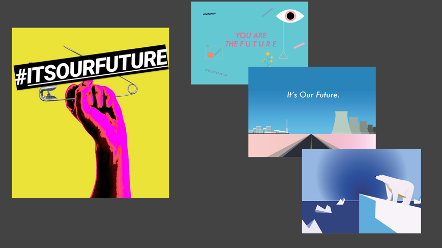
\includegraphics{Images/7/iof-3.png}
    \caption{Slides from the pitch deck we presented to The Charity, showing example interactions, a general structure, and visual ideas.}
    \label{fig:iof-pitch}
\end{figure}

Whilst safeguarding is undeniably integral to a project like this, we were keen to establish an approach to safeguarding that utilised The Charity's expertise as an organisation that works to protect and support young people. The project team (with myself at the lead) had a good deal of experience of creating safe, healthy, and comfortable places for young people to exist within, and we hoped The Charity could support us by filling in gaps in our experience or capacity.  At the outset of the project, The Charity had promised us a dedicated member of staff to deal with safeguarding concerns during the project, which we had made a condition of our engagement. In the pitch meeting, discussion quickly fixated on the use of specific digital technologies within the project, the degree to which they were perceived to be ‘safe’ technologies, and whether The Charity's use of these technologies might cause reputational issues for them. Around six months prior to the project, for example, The Charity had campaigned against TikTok for the ways it felt that it put young people at risk of sexual exploitation (due to the ability for anyone to livestream from it). A large part of conversation on the day then focused on whether TikTok was a viable platform for The Charity to be associated with given this campaign. They were tightly focused on the possibility of TikTok usage in the project causing them reputational damage by going against their previous campaigning. We agreed to not use TikTok within the project. The dynamics of justification and performativity re-presented themselves here - although the discussion theoretically started around online safety, the actual reasons given for not using TikTok were not that it might put young people in harm's way, but that it might make The Charity look bad to use TikTok after having campaigned against it. 

Similarly, a large amount of discussion focused on our potential use of Discord. The majority of The Charity's staff involved with the project (including Martin) had never heard of Discord. As such, the were incredibly uncertain about using it as they viewed it was inherently riskier. We presented some proposals for how we would monitor and moderate conversation, and hoped that we could draw upon The Charity's safeguarding capacity to support in the case of any disclosures of safeguarding issues or any harmful behaviours being exhibited. Yet despite our want to develop a collaborative approach to safe and healthy use of these social media platforms, discussion quickly trended towards bureaucratic and procedural issues - for example, The Charity weren't sure whether they had a risk assessment for the use of the platform. The concern around this risk assessment was not out of a desire to engage in a relational and ethical safeguarding practice, but instead a desire to ensure that The Charity would be legally and reputationally covered if they followed this approach.

It is tempting to take The Charity’s concern around safeguarding here in good faith – that they are an organisation that advances the cause of the rights and safety of children and young people and thus want to ensure that they can create and maintain safe spaces for them. Yet it became ever clearer throughout what followed that the The Charity's primary concerns were on reputation management. Their concerns were less about protecting children and young people (though undoubtedly they did care about this too) but instead protecting their reputation as a charity that occupies a central role in public influencing around the delivery of support services to children and young people. Even in approaching my research group in the first place, The Charity were hoping to accumulate discursive capital by positioning themselves as digitally innovative, excellent at partnership-working, and as the main guardian of the voices and experiences of children and young people. Immediately, the very things that might have led to an "innovative" project were what became imagined issues.

I was aware at this stage that I was caught in some of the dynamics that my participants who were frontline workers found themselves in frequently. Just like them, I was finding my good intentions compromised by a system that insisted on a high degree of bureaucratic, procedural, or representational work in order to do anything. I could recognise that I was being caught inside justification practices, and despite an awareness of these forces I found myself beginning to acquiesce to them. Initially, we set about trying to reassure The Charity that it could be possible to run the project safely and well - that we would be able to control and moderate interactions, ensuring nothing ‘bad’ or unintended would happen. Of course, this is not something that we would have been able to control, and indeed, some of what The Charity were looking for from moderation would reduce the possibility of participants in the project meaningfully connecting with each other and imagining and building futures collectively. We found ourselves caught in discussions around the kinds of young people who might be brought into the project, entering into discussions with The Charity about what "vulnerability" meant here and how we would ensure that participants were suitably vulnerable. In order to reassure them about the safety of the project, they asked me to document all of the possible touchpoints within the project, in order to ascertain that it would be possible to mitigate risk. I therefore set about creating an in-depth process diagram of the entire project (shown in figure \ref{fig:iof-process}) to highlight interaction touchpoints so that The Charity would be sure that we could triage any potentially concerning disclosures to them, and that we would otherwise be monitoring the chat. 

\begin{figure}[hbt!]
    \centering

% 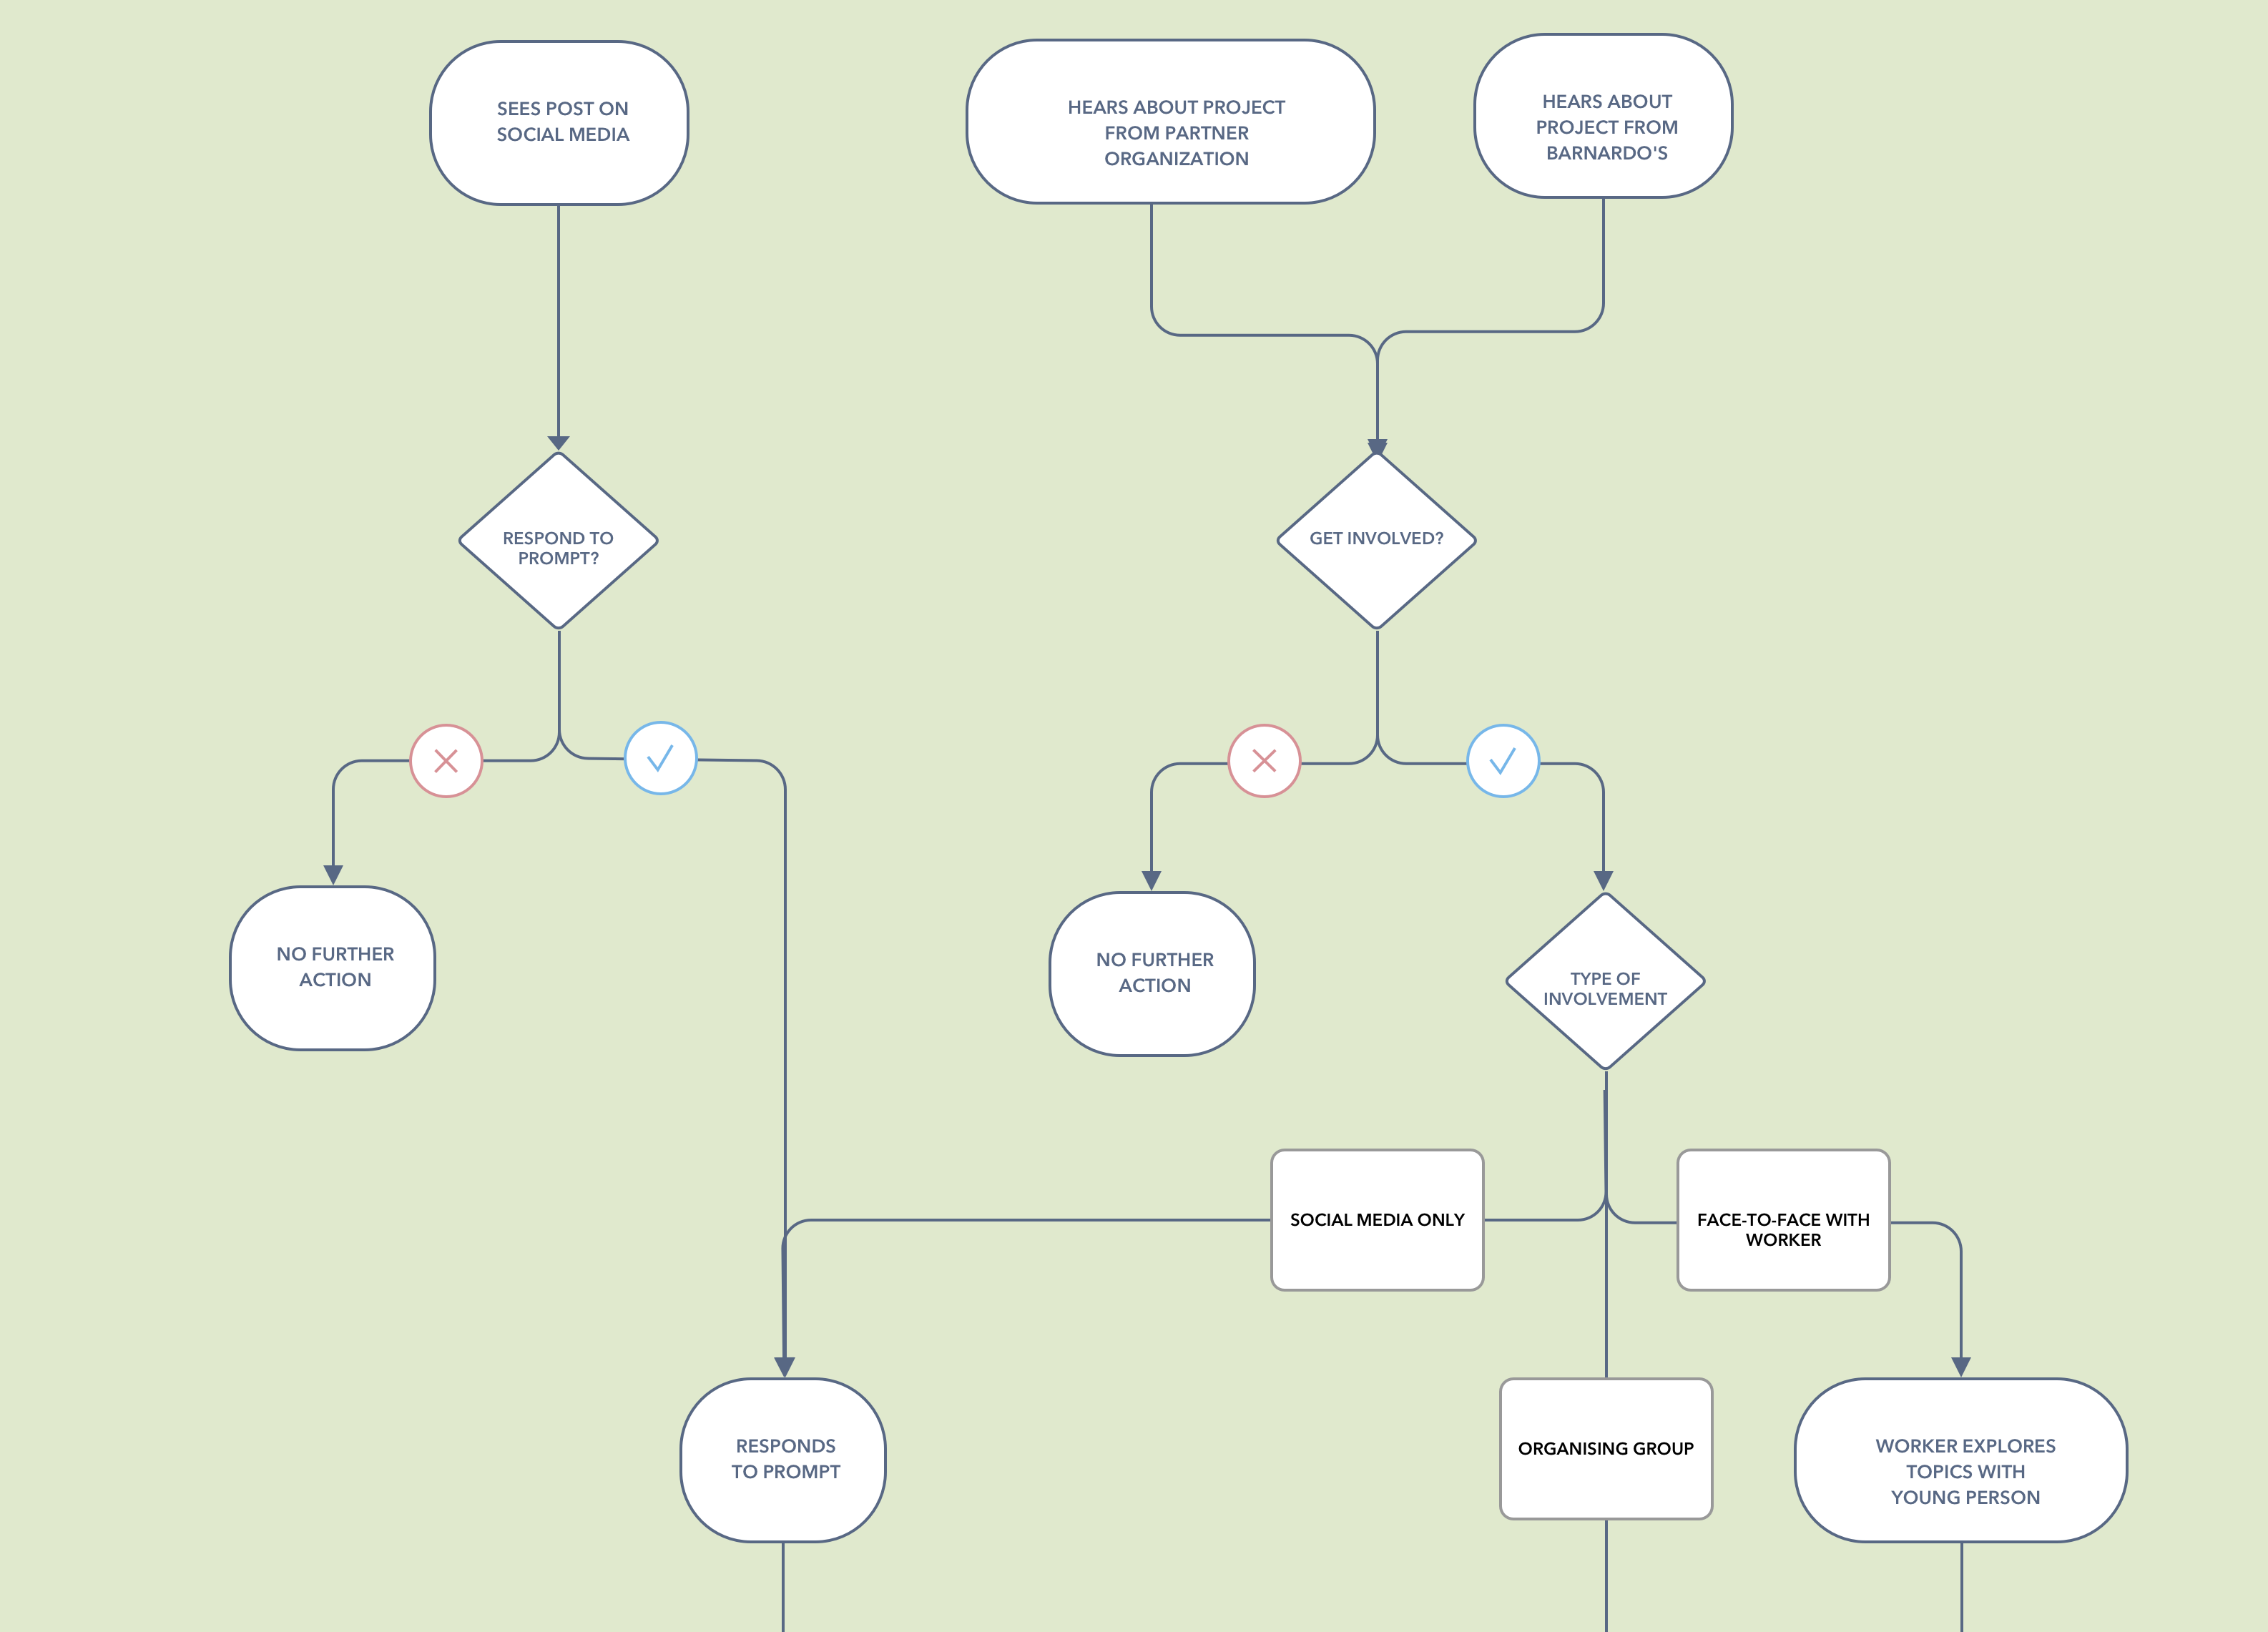
\includegraphics[rotate=90, width=1\linewidth]{Images/7/process-1a.png}
% 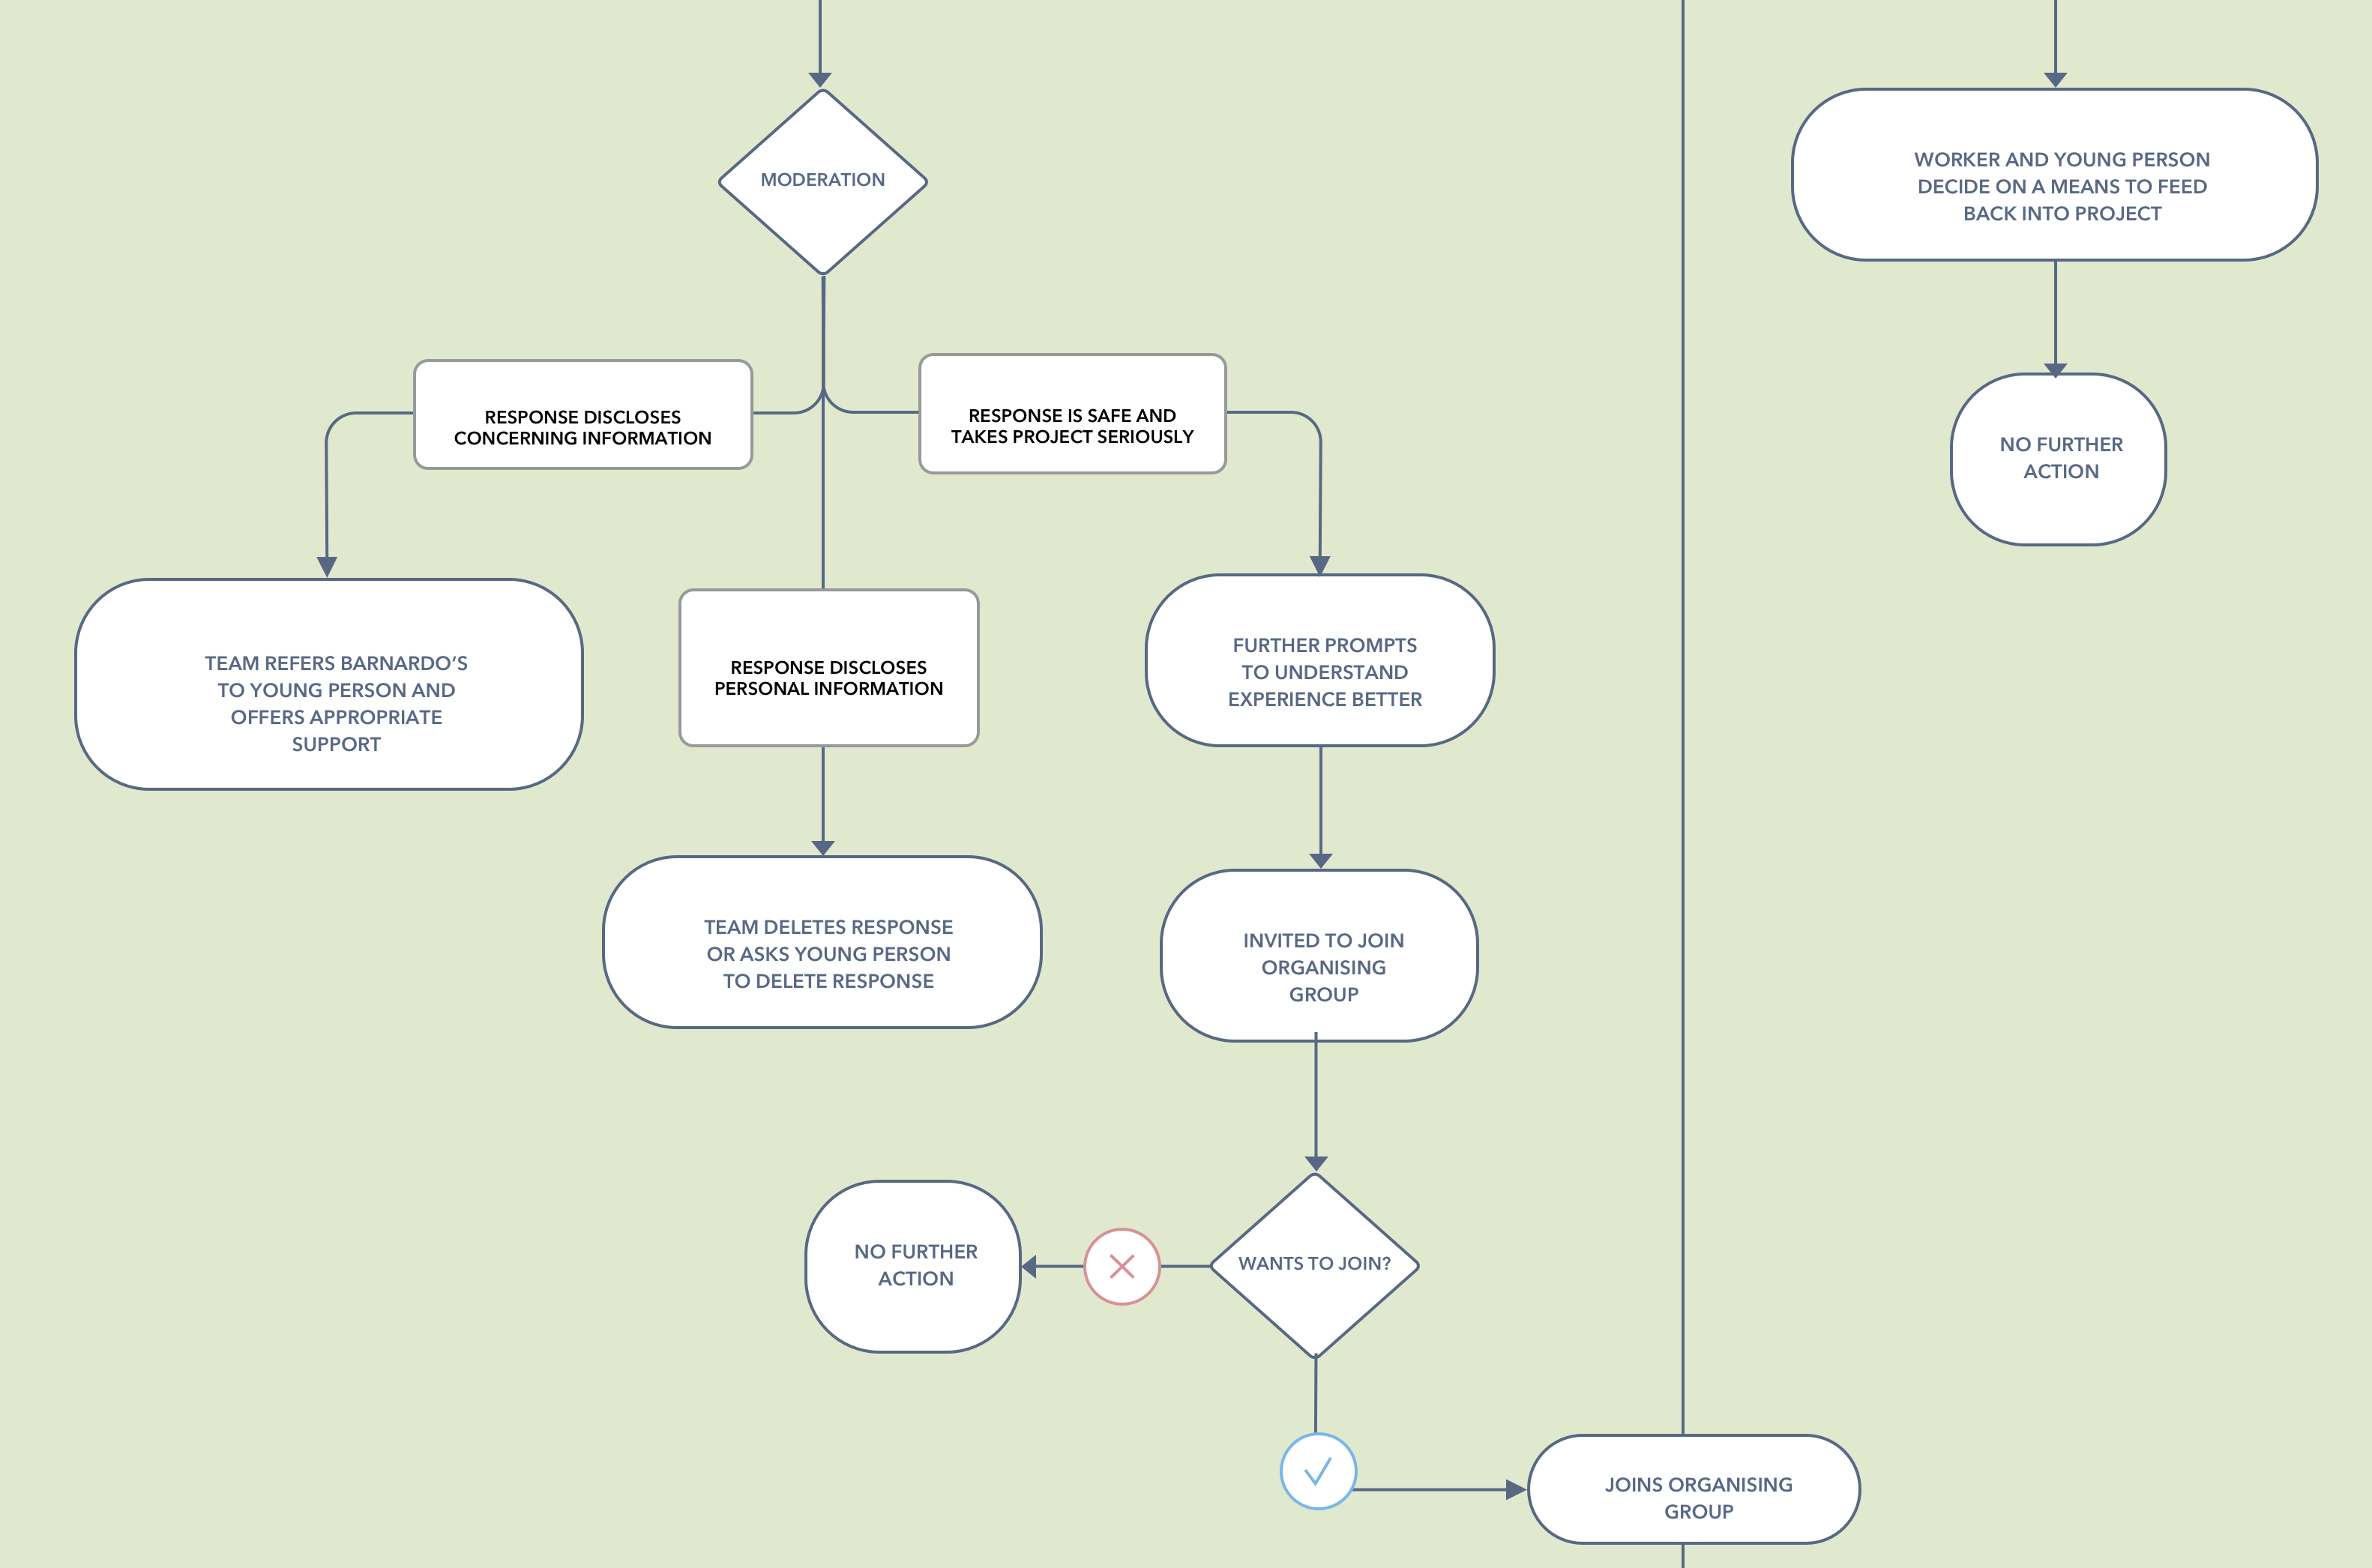
\includegraphics[rotate=90, width=1\linewidth]{Images/7/process-1b.png}
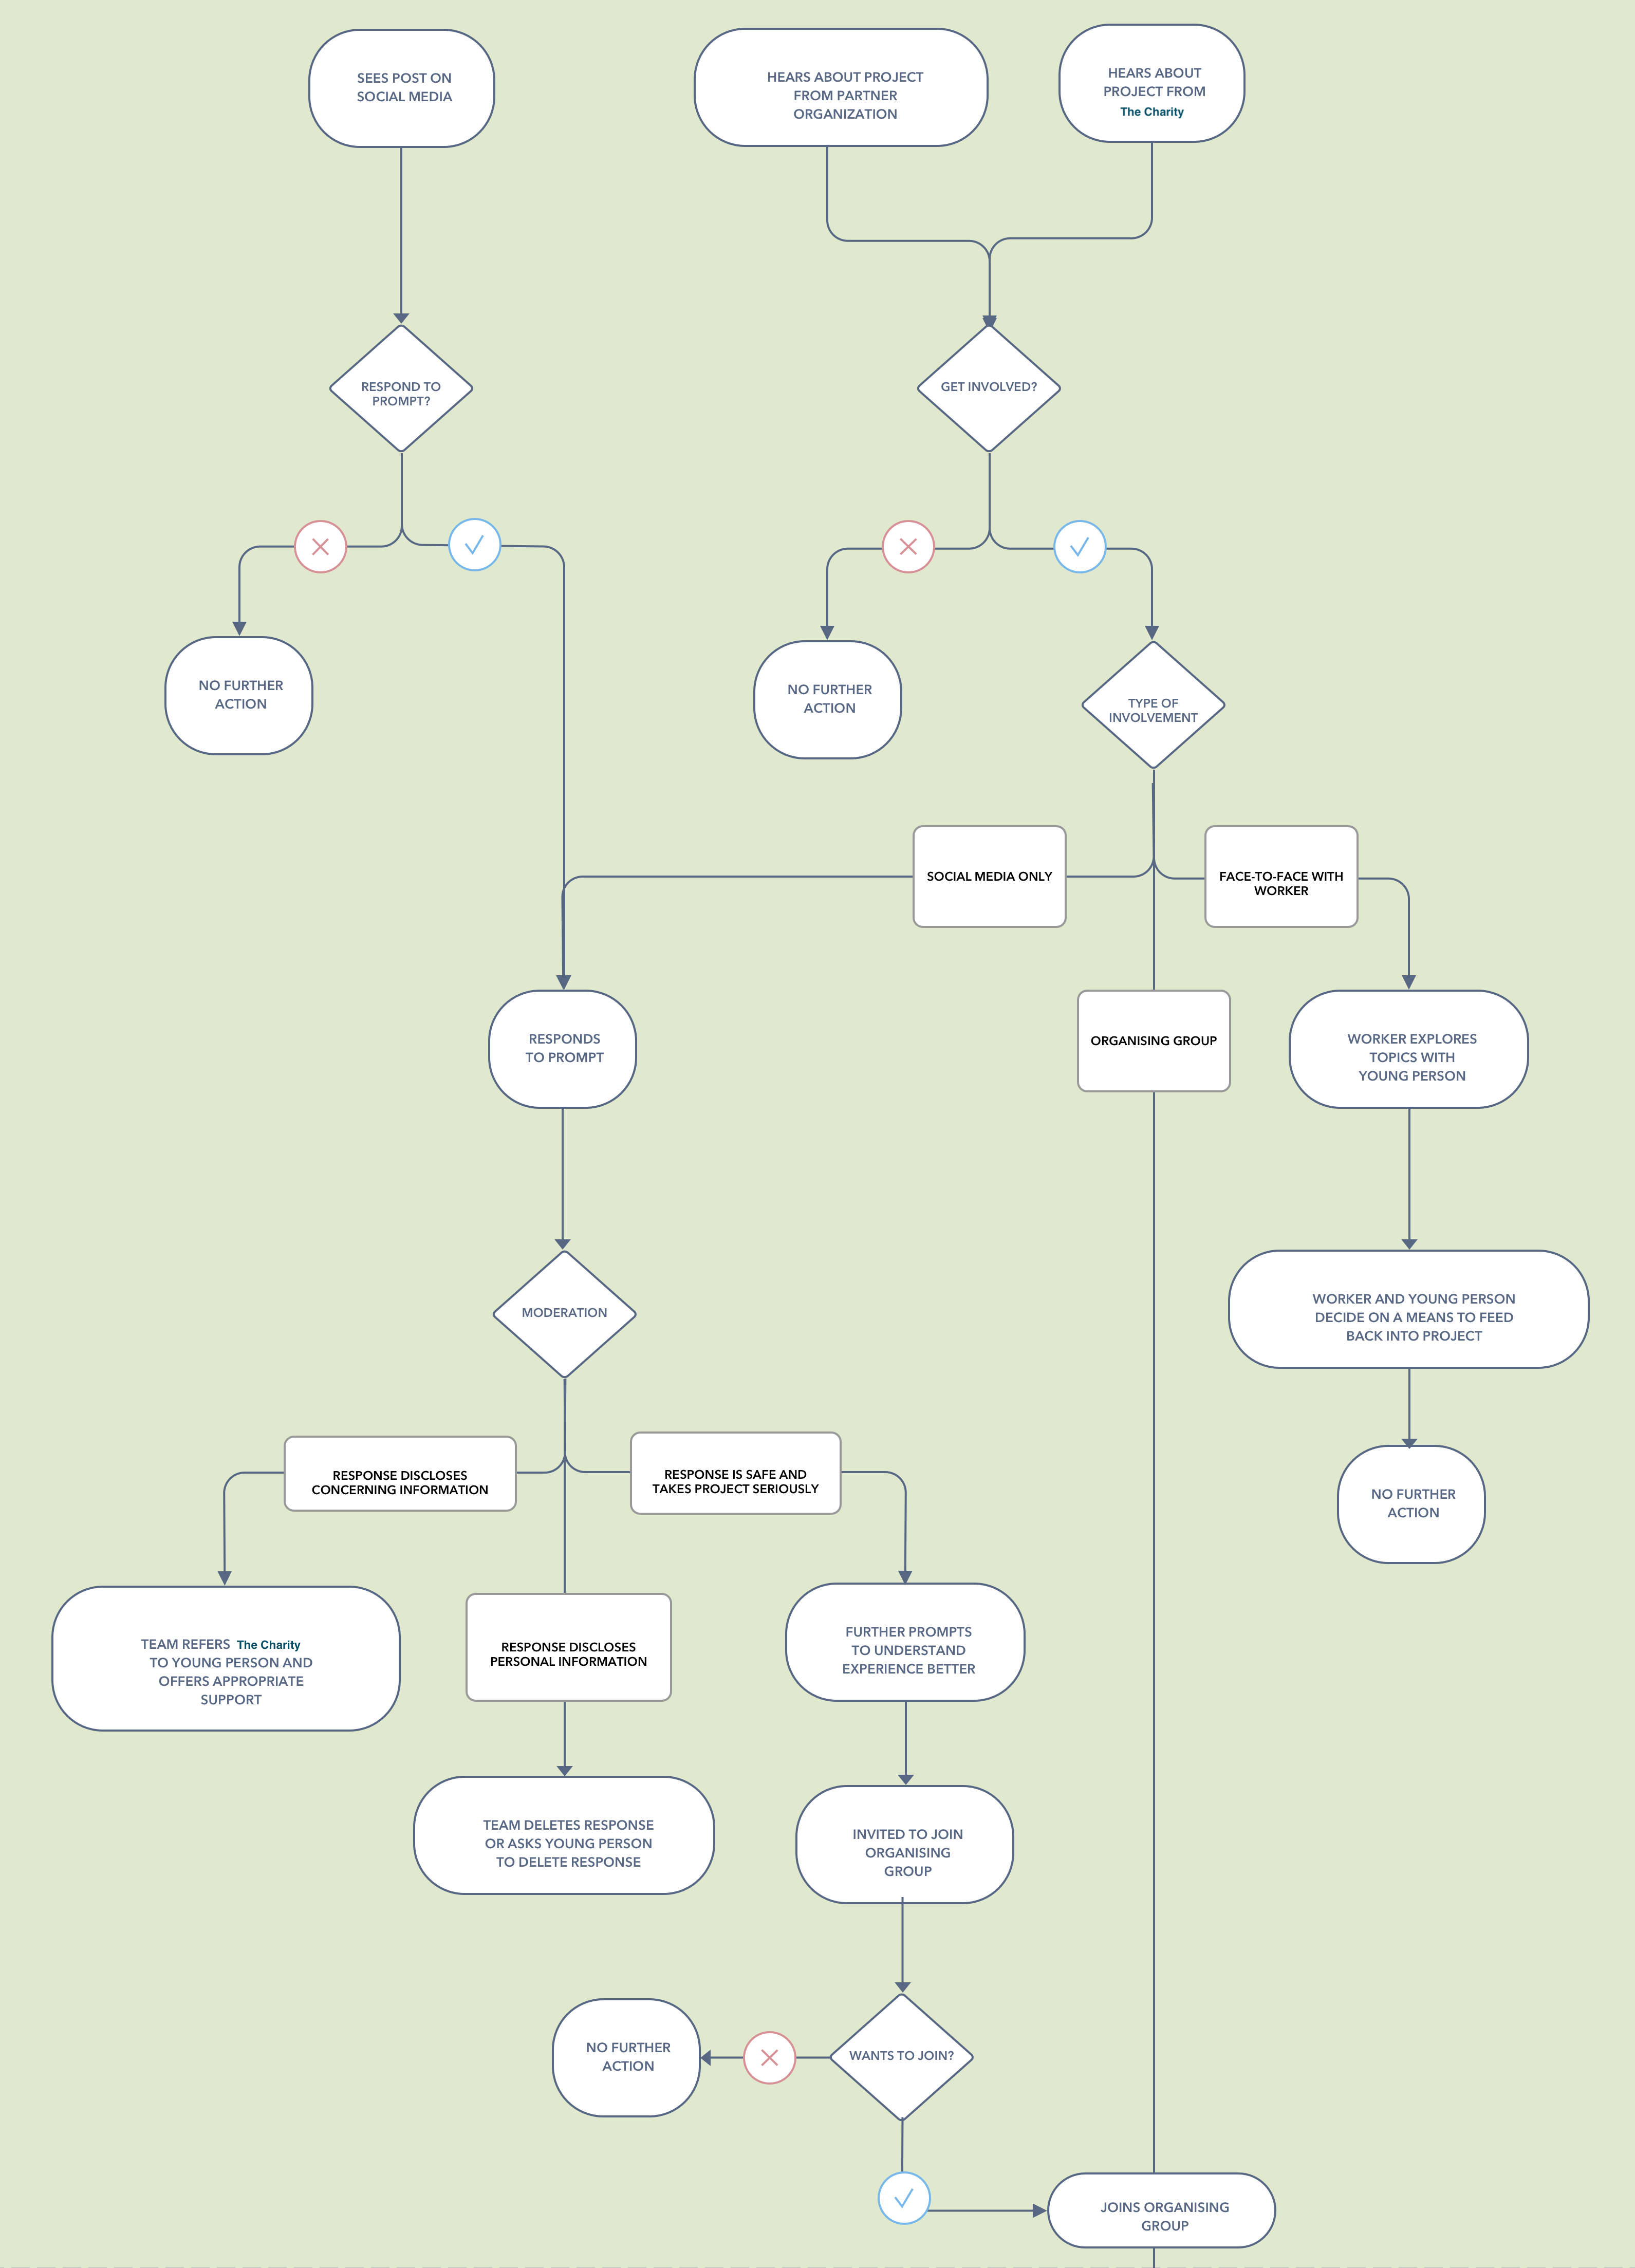
\includegraphics[width=1\linewidth]{Images/7/process-1.png}
    \caption{A diagram of the different potential touchpoints within the digital conversation iteration of the project. These are particularly structured around mitigating personal disclosures, at The Charity's behest (continues on next page).}
        \label{fig:iof-process}
    \end{figure}
\begin{figure}
    \centering
\ContinuedFloat
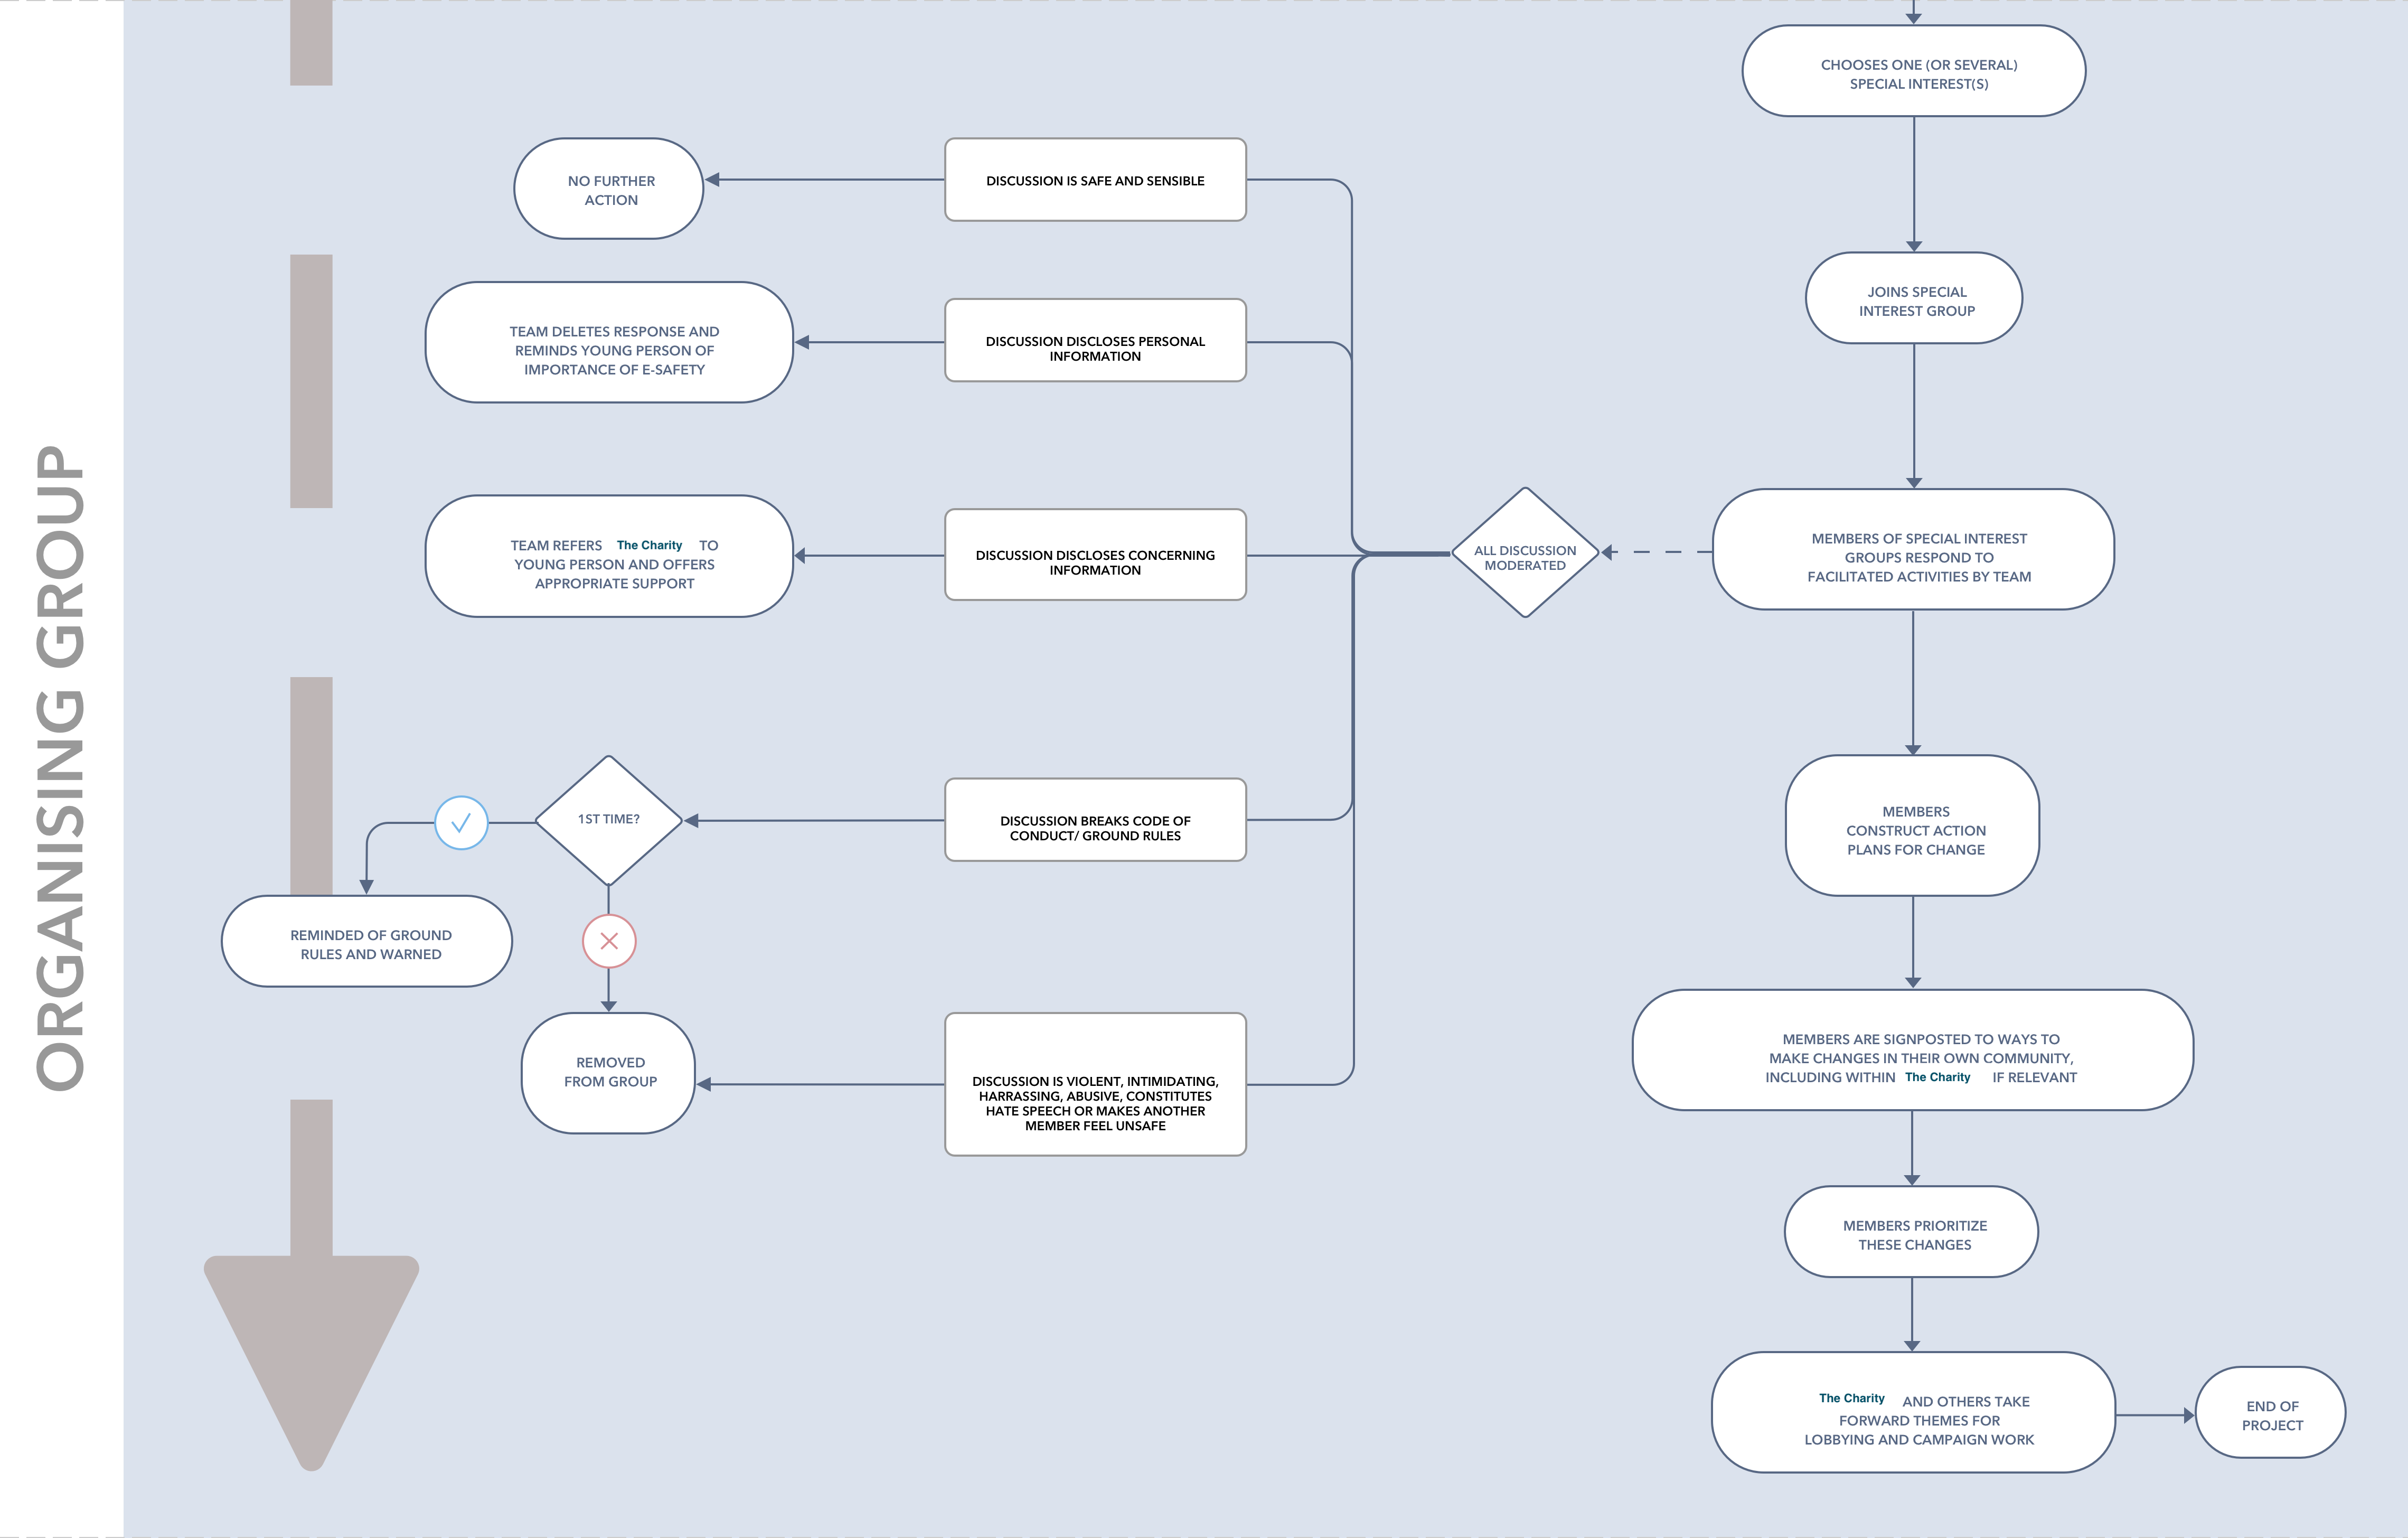
\includegraphics[angle=90, width=1\linewidth]{Images/7/process-2.png}
    \caption{A diagram of the different potential touchpoints within the digital conversation iteration of the project. These are particularly structured around mitigating personal disclosures, at The Charity's behest (continued).}
    \label{fig:iof-process}
\end{figure}


The Charity had created an environment of artificial scarcity. They had contacted us about the project with less than two months to go until its intended \textit{end}, setting a fixed deadline that was soon in the future because the project needed to be completed before Martin left the organisation. This time scarcity was then compounded as they brought in a number of bureaucratic and procedural issues which took significant amounts of working time, increasing the work that had to be done inside of this tight time-frame, and then frequently trying to accelerate our working pace.  I found myself switching between roles to attempt to satisfy The Charity’s increasingly large demands. I had to play project manager, interaction designer, service designer, researcher, youth worker, and safeguarding lead. I had to constantly switch between all of these roles. The work also began to creep into my personal life – I found myself working later and longer hours in order to try to get things ready in time. I created the aforementioned process diagram whilst on a family holiday where I had made clear that I did not intend to work. Martin called me several times throughout the holiday despite this, raising new issues that had emerged or explaining developments within the team, and I found myself working on the holiday in an attempt to keep the project going, making the process diagram in the back of my dad's car whilst my family went to get ice cream. Whilst this was in part due to my own lack of work boundaries at the time, this was a pattern of behaviour that I had witnessed in many of my participants, and it feels important to note this here too. Even at the time, I was aware just how much I found myself mirroring the behaviours of the workers I observed in chapters \ref{ch:5} and \ref{ch:6} - slipping between multiple roles, working all the time, becoming increasingly burnt out whilst I produced justificatory documents like process diagrams, multiple rounds of ethical approval documents to The Charity's internal ethical review board, and trying to find a visual style for the project that The Charity felt they could support. 

We faced increasing resistance from The Charity as we moved into the development of a visual identity for the project - again moving into the discursive, performative space of imagery. Though our initial pitch to The Charity had included a solidarity fist as the project's logo, and they were on board with our reasoning for this (creating a visual style that suggested a protest-like movement for young people), once we presented them with some logo materials for approval (shown in figure \ref{fig:iof-logo-1}), we were met with pushback. Martin shared that the senior leadership team felt that the logo looked "uncomfortably close to a fist and that is obviously not what we or you are about…", inviting us to think of "another arresting image which couldn’t be misinterpreted in that way?", though there is a clear distinction between a palm-facing fist of solidarity and a closed fist of aggression. Then Martin began to become concerned that \textit{It’s Our Future }was too generic a name, wanting to go with their initial choice of \textit{OurFutureOurUK} in order to make it "more upfront that this is seeking input and energy from across all four corners of the country plus… appropriating a term in ‘UK’ that too often gets used/abused by extreme right wing. It’s our nation not theirs". Using the language of `concern', The Charity wanted to sanitise the image of the project and remove some of the more explicitly political content.

\begin{figure}[hbt!]
    \centering
    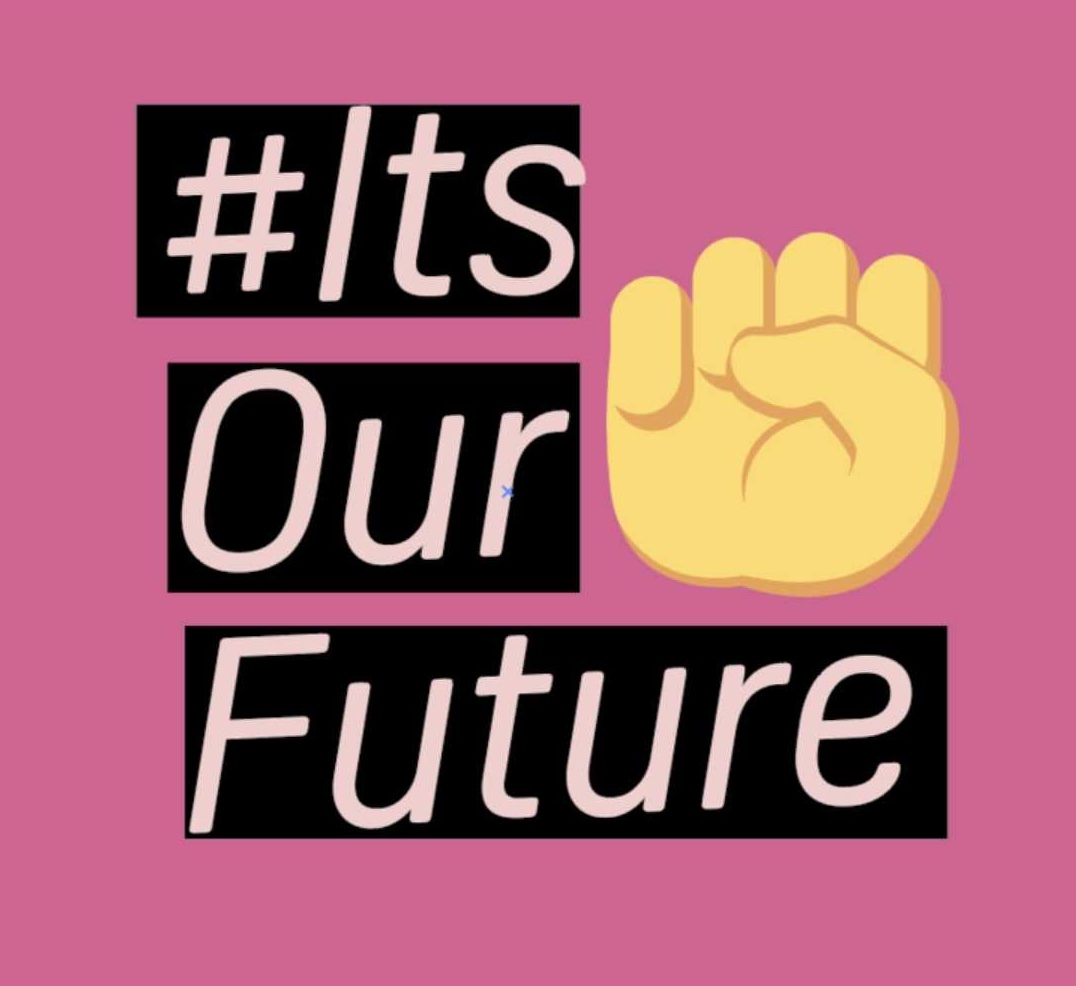
\includegraphics[width=0.25\linewidth]{Images/7/iof-logo-1.png}
    \caption{Our initial logo design for \textit{It's Our Future}}
    \label{fig:iof-logo-1}
\end{figure}

We continued trying to appease The Charity despite the breakdown in communication and collaboration. Although we were uncomfortable with using their choice of name, as we felt it perpetuated rather than reclaimed the use of ‘UK’ rather than the extreme right wing, we found a compromise by creating a new logo which emphasized the UK within it and disposed of the solidarity fist.  This logo was still met with further resistance by Martin's team, as they were concerned that "the ‘hashtag’ obscures too much of Wales". In the final design (pictured in figure \ref{fig:iof-logo-2}) we moved the title and changed the colouring of the Republic of Ireland (so as to make clear it was not included within the scope of the project, as we anticipated this could be a further comment). We were becoming increasingly concerned about the level of granularity of the comments. Quibbling over small representational details was diverting our attention from making progress on the actual design of the activities that participants would engage in. As we were settling these discussions, a longer email arrived from Martin that made us decide to pause the project as it currently was.
\begin{figure}
    \centering
    
\includegraphics[width=0.25\linewidth]{Images/7/iof-logo-2.png}
    \caption{Our final logo design for \textit{It's Our Future}, incorporating The Charity's changes}
    \label{fig:iof-logo-2}
\end{figure}
More than halfway through the project, Martin's email asked us:
\begin{itemize}
\item For a copy of our safeguarding policies,
\item Whether there was any learning that the research group had picked up from safeguarding challenges with other organisations,
\item To take responsibility for ensuring that any organisations we contacted would comply with our safeguarding policy,
\item To make explicit in promotional materials that the project was not the place for highly personal disclosures, and
\item To include an age-verification process in the Discord phase of engagement.
\end{itemize}
We were taken aback by such foundational questions or suggestions of changes just two and a half weeks before the project was going to be live. We had been raising questions around much of this throughout, so this new set of requirements at this stage felt like one thing too many. It felt as if The Charity were trying to push the legal responsibility for the project onto us, and thus the University. Obviously this is not a commitment that I could make as a PhD student, so I spoke with my supervisors and the heads of my research group, and we agreed that the process would be unable to go ahead in its current form. The Charity had ignored our repeated requests for them to either handle the safeguarding component of the project, or at least train our project team. We responded to Martin's email explaining that we were unable to meet their requests - that in previous projects, we had followed the safeguarding approaches of our partner organisations, that whilst the University has safeguarding policies, there is little training in how to employ these, and our inability (and unwillingness) to create an age-verification process within the Discord phase of the engagement, as there is no reliable way to verify the age of young people online. We explained that there was no way to sort the issues with the project in the amount of time available, and that we would need to find an alternate way forward. 

At this stage, I took a moment to reflect on just how enmeshed in justification practices we had become in our attempt to make the project happen. We had made little progress on the original aims of the project as we had become tied up in the aforementioned bureaucratic back-and-forth. Whilst I had wanted to see how a project like this could be used to develop methods to work against austerity-intensified capitalist realism, I had instead found myself caught up in justification, classification, and discursive accumulation practices. Martin suggested that instead of a digital conversation with an in-person `launch' event for a manifesto, it might make more sense for us to use that in-person event as a large-scale design workshop, through which we might create the manifesto. We agreed that this was a useful way forward, and revisited our original ideas for the project to see how we could transform the work we had been preparing for the digital conversation activities into in-person activities in a design workshop. We returned to the core structure for the project: attempting to enhance the counterpower of young people perceived to be vulnerable, as they went through the stages of articulating problems, building power, confronting those with traditional power, and maintaining power, drawing upon the emergent strategy elements and research justice where useful. 

Although justification practices continued to appear throughout this stage of the project too, our issues were less significant and we were able to more confidently advocate for our approach. The final context for \textit{It's Our Future}, then, was to be an in-person workshop, bringing together young people, frontline workers, and `civic leaders', supporting young people to reflect on what could change their lives, identify reasons why those things hadn't yet changed, imagine futures where those changes have been made, and identify a pathway towards making those futures. From the digital conversation iteration of the project and our experience with justification practices, we brought several project aims forward:
\begin{itemize}
\item Having a simple ask that could be answered from lived experience,
    \item Building critical consciousness/idea counterpower, to help transform this simple ask into a clearer articulation of the political and social problems that underpinned that experience,
    \item Building physical counterpower through the exchange of skills and resources,
    \item Ensuring the overall process centered on building trusting relationships,
    \item Ensuring that imagining and meaningfully inhabiting collective potential futures was at the heart of the experience,
    \item Emphasising the ability of all present to make material changes at different scales,
    \item Providing opportunities to safely confront oppression,
    \item Leveraging situated sense-making to avoid the reinterpretation of ideas by those without lived experience, and
    \item Avoiding justification practices and discursive accumulation taking root. 
\end{itemize}
With these aims in mind, we began to redesign \textit{It's Our Future} as an in-person, large-scale workshop.

\section{The final project: supporting people to imagine alternative futures }
\label{sec:7-5-final}
We structured the in-person workshop by creating four activities, with each taking about an hour. Developing on our approach to the digital conversation, these activities were intended to begin from a simple ask based on lived experience, identify the ways that this was different from the world as it currently exists, imagine a future where those changes have taken place, and identify steps that could be taken to go from how things are now to the imagined future world. These four activities were entitled:
\begin{itemize}
    \item What would transform your life?
    \item How are things now?
    \item Dreaming the future
    \item Building the future
\end{itemize}
In this section, I will describe each of these activities in turn and the key design considerations behind these. In section \ref{sec:7-6-understanding}, I will describe what happened when we ran these activities, who attended the workshop, and how the methods worked.

\subsection{What would transform your life?}
This activity was structured around the use of idea cards (shown in figure \ref{fig:idea-cards}). These were \textit{It's Our Future} branded cards which were blank on the front. I chose to style these after tarot cards, as there was an easy visual reference in the act of laying cards down sequentially to attempt to speak about the future.  Though initially created as playing cards, tarot cards are typically used as a divination tool, in which a person is given a `reading' of their future via the drawing of multiple cards. We essentially used these cards like sticky notes might be used in other design workshops, as an easy way to record information as it arises. Partly, this was as pragmatic research concern - as we knew there were likely to be around 100 people attending the workshop, we wanted to ensure that there was an easy way to record data for the project and not have insights get lost in conversation. We also wanted to prioritise situated sense-making, and the ability of communities with lived experience of an issue to make their own analyses of what issues they are facing and what should be done about that. 

\begin{figure}
    \centering
    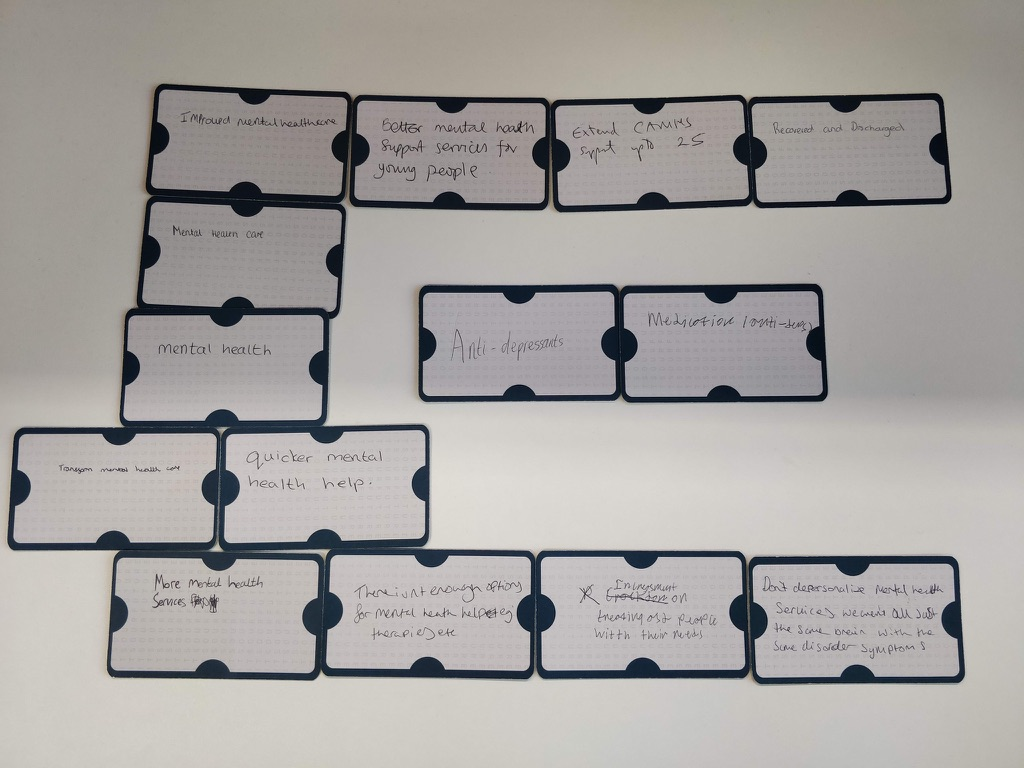
\includegraphics[width=1\linewidth]{Images/7/idea-cards.jpeg}
    \caption{The idea cards used in \textit{It's Our Future} during the post-event analysis}
    \label{fig:idea-cards}
\end{figure}

Whilst creating this activity, we envisioned it as a card game, but it would be more accurate to refer to it as a playful facilitation aid. We asked participants to write answers to the question "what would genuinely transform your life if it happened in the next five years?" on three blank idea cards, one idea per card. These cards were then collected in, shuffled, and dealt back out to them. At this point, participants would have a hand of cards of ideas of what other people around the table felt would change their lives if they happened in the next five years. Taking it in turns, participants could then either:
\begin{itemize}
    \item Play a card, explaining why someone might think that would change their life, or
    \item Connect a card, explaining why the two issues they are connecting are related.
\end{itemize}
If they didn’t have cards in their hand on their turn (because they had played all of their cards), then they could either:

\begin{itemize}
    \item Connect a card, explaining why the two issues they were connecting are related, or
    \item Discard a card, explaining why it’s less related to the other ones.
\end{itemize}

When participants decided they were happy with the cluster on the table – and they had gone for an entire round without any participant wanting to change any aspect of the clusters – they had formed a set of priorities for the futures they would be imagining that day. 

The cards were designed to suggest this connecting behaviour, as the edge of each card featured semi-circles so that when they were joined they would form a complete circle. Beginning with a simple ask that directly concerned participants' lived experiences ensured everyone would be able to participate without having a sophisticated analysis of what might make their lives better. By shuffling and re-dealing the cards and building the `game' around explaining why issues were related, the `game' served to build empathy and solidarity between participants, as they knew that someone at the table felt this issue to be important, and to think about why someone might think of this as important. This quickly built trust and rapport between participants. It also helped groups to identify shared issues of concern and broaden their understanding of these issues. For example, someone might have connected a card saying "Get a car" to a card saying "Have more freedom and independence". By connecting these cards, a desire for personal transport becomes attached to the wider idea of freedom and independence. This supported the groups to analyse their own data and define their own parameters for the rest of the day's activities. At the end of this activity, participants wrote on summary cards (shown in figure \ref{fig:summary-cards}) to synthesise their card clusters into a maximum of three more nuanced issues which represented changes that the whole group felt would transform their lives if it happened in the next five years. Summary cards also acted as a useful reset, ensuring that the rest of the cards could be moved away from the `play space' on the table.

\begin{figure}[hbt!]
    \centering
    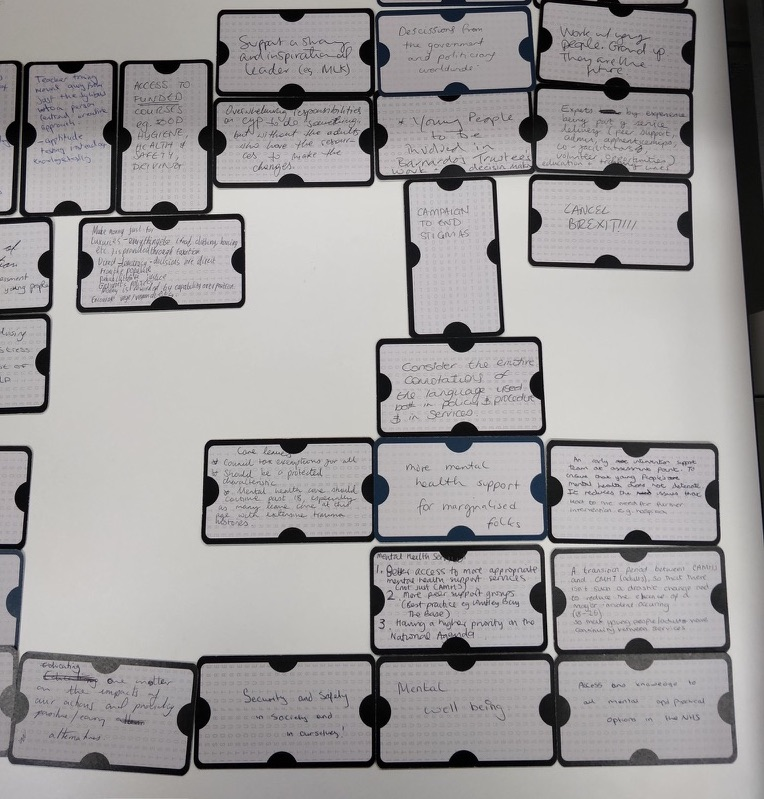
\includegraphics[width=1\linewidth]{Images/7/summary-cards.jpeg}

    \caption{An example of summary cards from \textit{It's Our Future} during the post-event analysis}
    \label{fig:summary-cards}
\end{figure}
\subsection{How are things now?}
Participants took their summary cards from the previous activity, and were invited to think about what might have led to these changes not having been made in the present. Specifically, they were invited to use these to think about potential pasts - to think backwards and imagine who or what might have been involved with making things be the way that they are right now. It was not important whether these ideas were actually why these changes hadn't been made, as the central intention of this activity was to introduce a sense of defamiliarisation, contingency, and possibility. Thinking back to the core idea of capitalist realism, this activity was intended to interrupt the idea that capitalism is the only viable political and economic system, and highlight the fact that our current sociopolitical state of being was constructed by historical actors making choices.

For example, if a group's shared concerns centred on climate change, then this activity would ask how the world might have arrived at a situation in which anthropogenic climate change was a threat to their futures, who might have been involved, and what they might have done. This activity was intended to create a sense of contingency and possibility. This activity supported groups to map out some of the actors and factors involved in the thing that they wanted to change, to give the futures that they would imagine in the next activity a material basis to arise from. To return to the climate change example, this might support the group to think about who has a vested interest in the continuation of the mass use of fossil fuels. As such, this activity also helped with the politicisation of the issues identified in the previous activity by supporting groups to relate them to their structural contexts, encouraging the development of critical consciousness and idea counterpower as groups created their own analysis of why the world is how it is. 
 
\subsection{Dreaming the future}
In this activity, participants were presented with everyday activities on prompt cards, such as "seeing a movie with friends", or "going on holiday", and asked to imagine how these these activities might be different in a world which had made the changes that they wanted for the future. The idea of this activity was to articulate a shared vision of the future and to ground this future in everyday activities, so that it didn't feel as if it was some distant, impossible fiction. Participants were encouraged to pick one or two of the summary cards and to think about how the activities on the prompt cards might be different in light of these. To return to the climate change example, it could be that in a world which isn’t threatened by imminent climate collapse, going to the cinema requires getting there in a form of public transport powered by renewable energy, or more community cinemas, so people had to travel less distance in order to reach the cinema.

\subsection{Building the future}
Using each of the activities that came before it, the final activity was grounded in getting participants to make the connections between their imagined future and what that felt like, and their experiences in the present. It was intended to help groups to think of the practical changes that could be made to get closer to that world by working forward from the ideas developed in `how are things now' and reaching towards the visions from `dreaming the future'. As groups were composed of young people, frontline workers, and civic leaders, this activity was informed by a variety of identities and positionalities. Participants identified the "next most elegant step" \citep[p. 220]{brown_emergent_2017}, a core aspect of emergent strategy practice, and wrote these on ‘Blueprint for the Future’ cards, taking these home with them as a reminder of their commitment to continued action. 

\section{Understanding the efficacy of the \textit{It's Our Future} methods}
\label{sec:7-6-understanding}
In October 2019, 45 young people and 40 frontline youth workers, managers, and civic leaders attended \textit{It's Our Future} at One Great George Street, just around the corner from the House of Commons in London. We divided them into groups of no more than ten, with a facilitator from the research team or The Charity guiding. On the day, I acted as a meta-facilitator, supporting each of the facilitators to run the process, and keeping the overall event together and on time. The event felt relatively successful - there was a great deal of energy and enthusiasm in the room, and throughout the course of the day participants expressed that they felt that they were being authentically listened to, that they had enjoyed talking about both personal and societal issues and "how we realistically could make this a better world for ourselves and for future generations". As the event seemed to have at least partially achieved its intentions, I turned towards inductively analysing these methods to understand what worked, how it worked, and how this could be developed upon. I reviewed the idea and summary cards that were produced through the course of the event, both in terms of the content that was on them and the developments and change in that content throughout the event (as I had collected the cards chronologically throughout the workshop). I also invited the facilitation team to share their reflections and notes with me, and drew upon these to understand how the methods worked and what might need to be changed about them to most effectively work against austerity-intensified capitalist realism. Finally, I compared these insights against the components of my grounded theory of justification, classification, and discursive accumulation practices to understand how these methods had influenced their functioning. As a result of this, I do not return to the aims identified in section \ref{sec:7-2-methods} explicitly, as I am more focused on understanding the limitations of the method in order to iterate on these and refine them further in the next chapter.

\subsection{Developing critical consciousness from lived experience}
\textit{It's Our Future} was most successful in the way that it supported participants to develop idea counterpower, or critical consciousness. In the first activity, the majority of things that people identified would transform their life if they happened were all relatively simple, typically consisting of a single word, a \textit{category} of change, or were conceptualised in terms of capital. For example, some of these initial cards (pictured in figure \ref{fig:idea-cards-eg}) simply read "graduate", "job", "driving", "house", "mental health", "climate change", "money" or "fame". In these cards from the first activity, there is not a sense of why participants might want these changes, what specifically within this category of change they might be looking for, or whether this would be a positive or negative change. Although this is not a perfect proxy for a participants' level of critical consciousness prior to the beginning of the workshop, it is the closest proxy available. 

\begin{figure}[hbt!]
    \centering
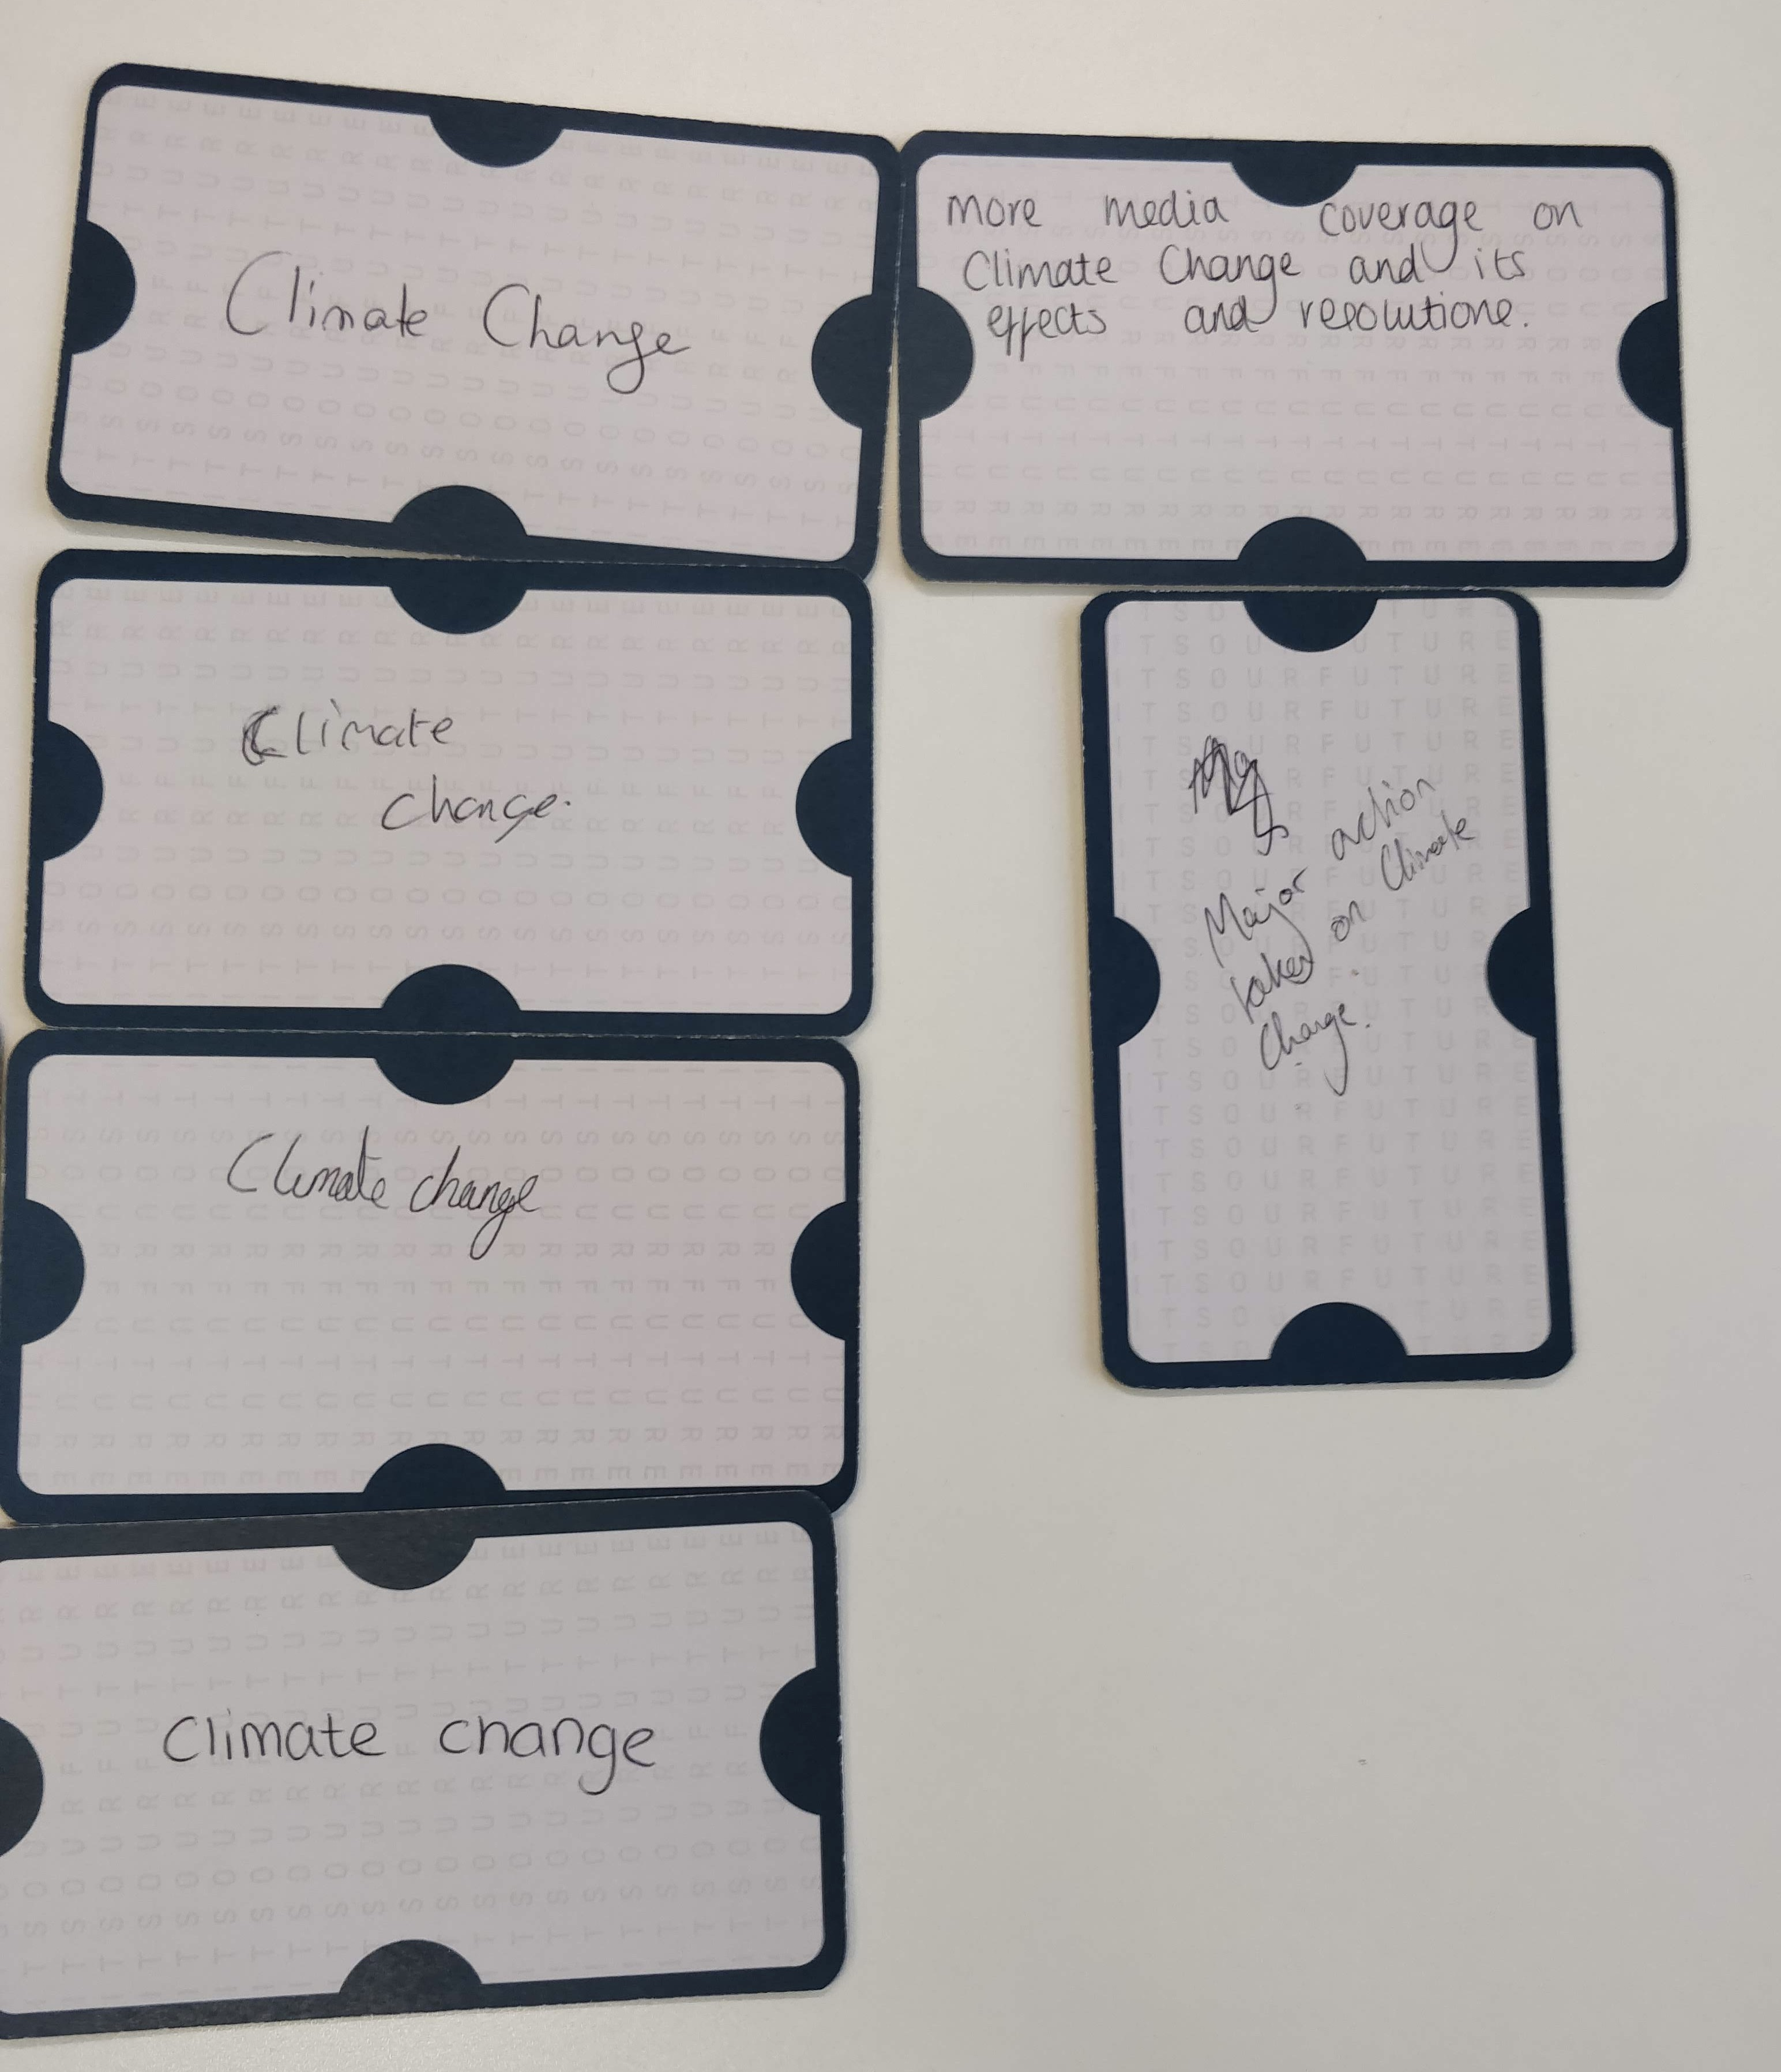
\includegraphics[width=0.8\textwidth]{Images/7/idea-cards-climate.jpeg}
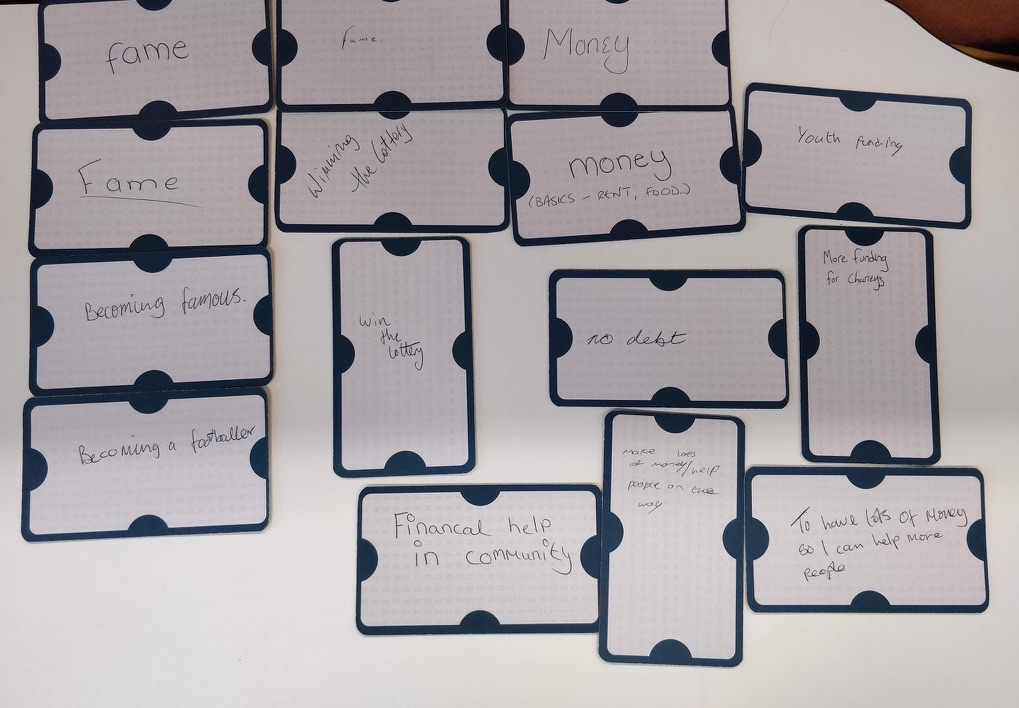
\includegraphics[width=0.8\textwidth]{Images/7/idea-cards-money.jpeg}
  \caption{A selection of idea cards from \textit{It's Our Future}, clustered by theme.}
    \label{fig:idea-cards-eg}
\end{figure}

By  the end of the workshop, the final summary cards (pictured in figure \ref{fig:summary-cards-eg}) contained a much clearer articulation of what the issue they were experiencing was, and what change they wanted to see to improve these issues. Taking the example of "climate change" again, throughout the course of the workshop these ideas developed into "Need to contact energy suppliers to see what changes they are making to go towards renewable energy" and "Create new adverts on the new renewable energy sources available". Whilst these aren't in themselves novel ideas, they represent a development in the minds of the people expressing them, moving from a simple articulation to one with greater direction and intention. Something like contacting an energy supplier could constitute a "next most elegant step", which is a huge change if someone entered the workshop feeling powerless about climate change. Similarly, something that had been expressed simply as "mental health" transformed into a discrete set of policy demands, including "Better access to more appropriate mental health support services", "More peer support groups", and "Having a higher priority on the National Agenda". There is a clear link being made between individual experiences and the changes in structural conditions that might be required for these individual experiences to shift. 

\begin{figure}
    \centering
    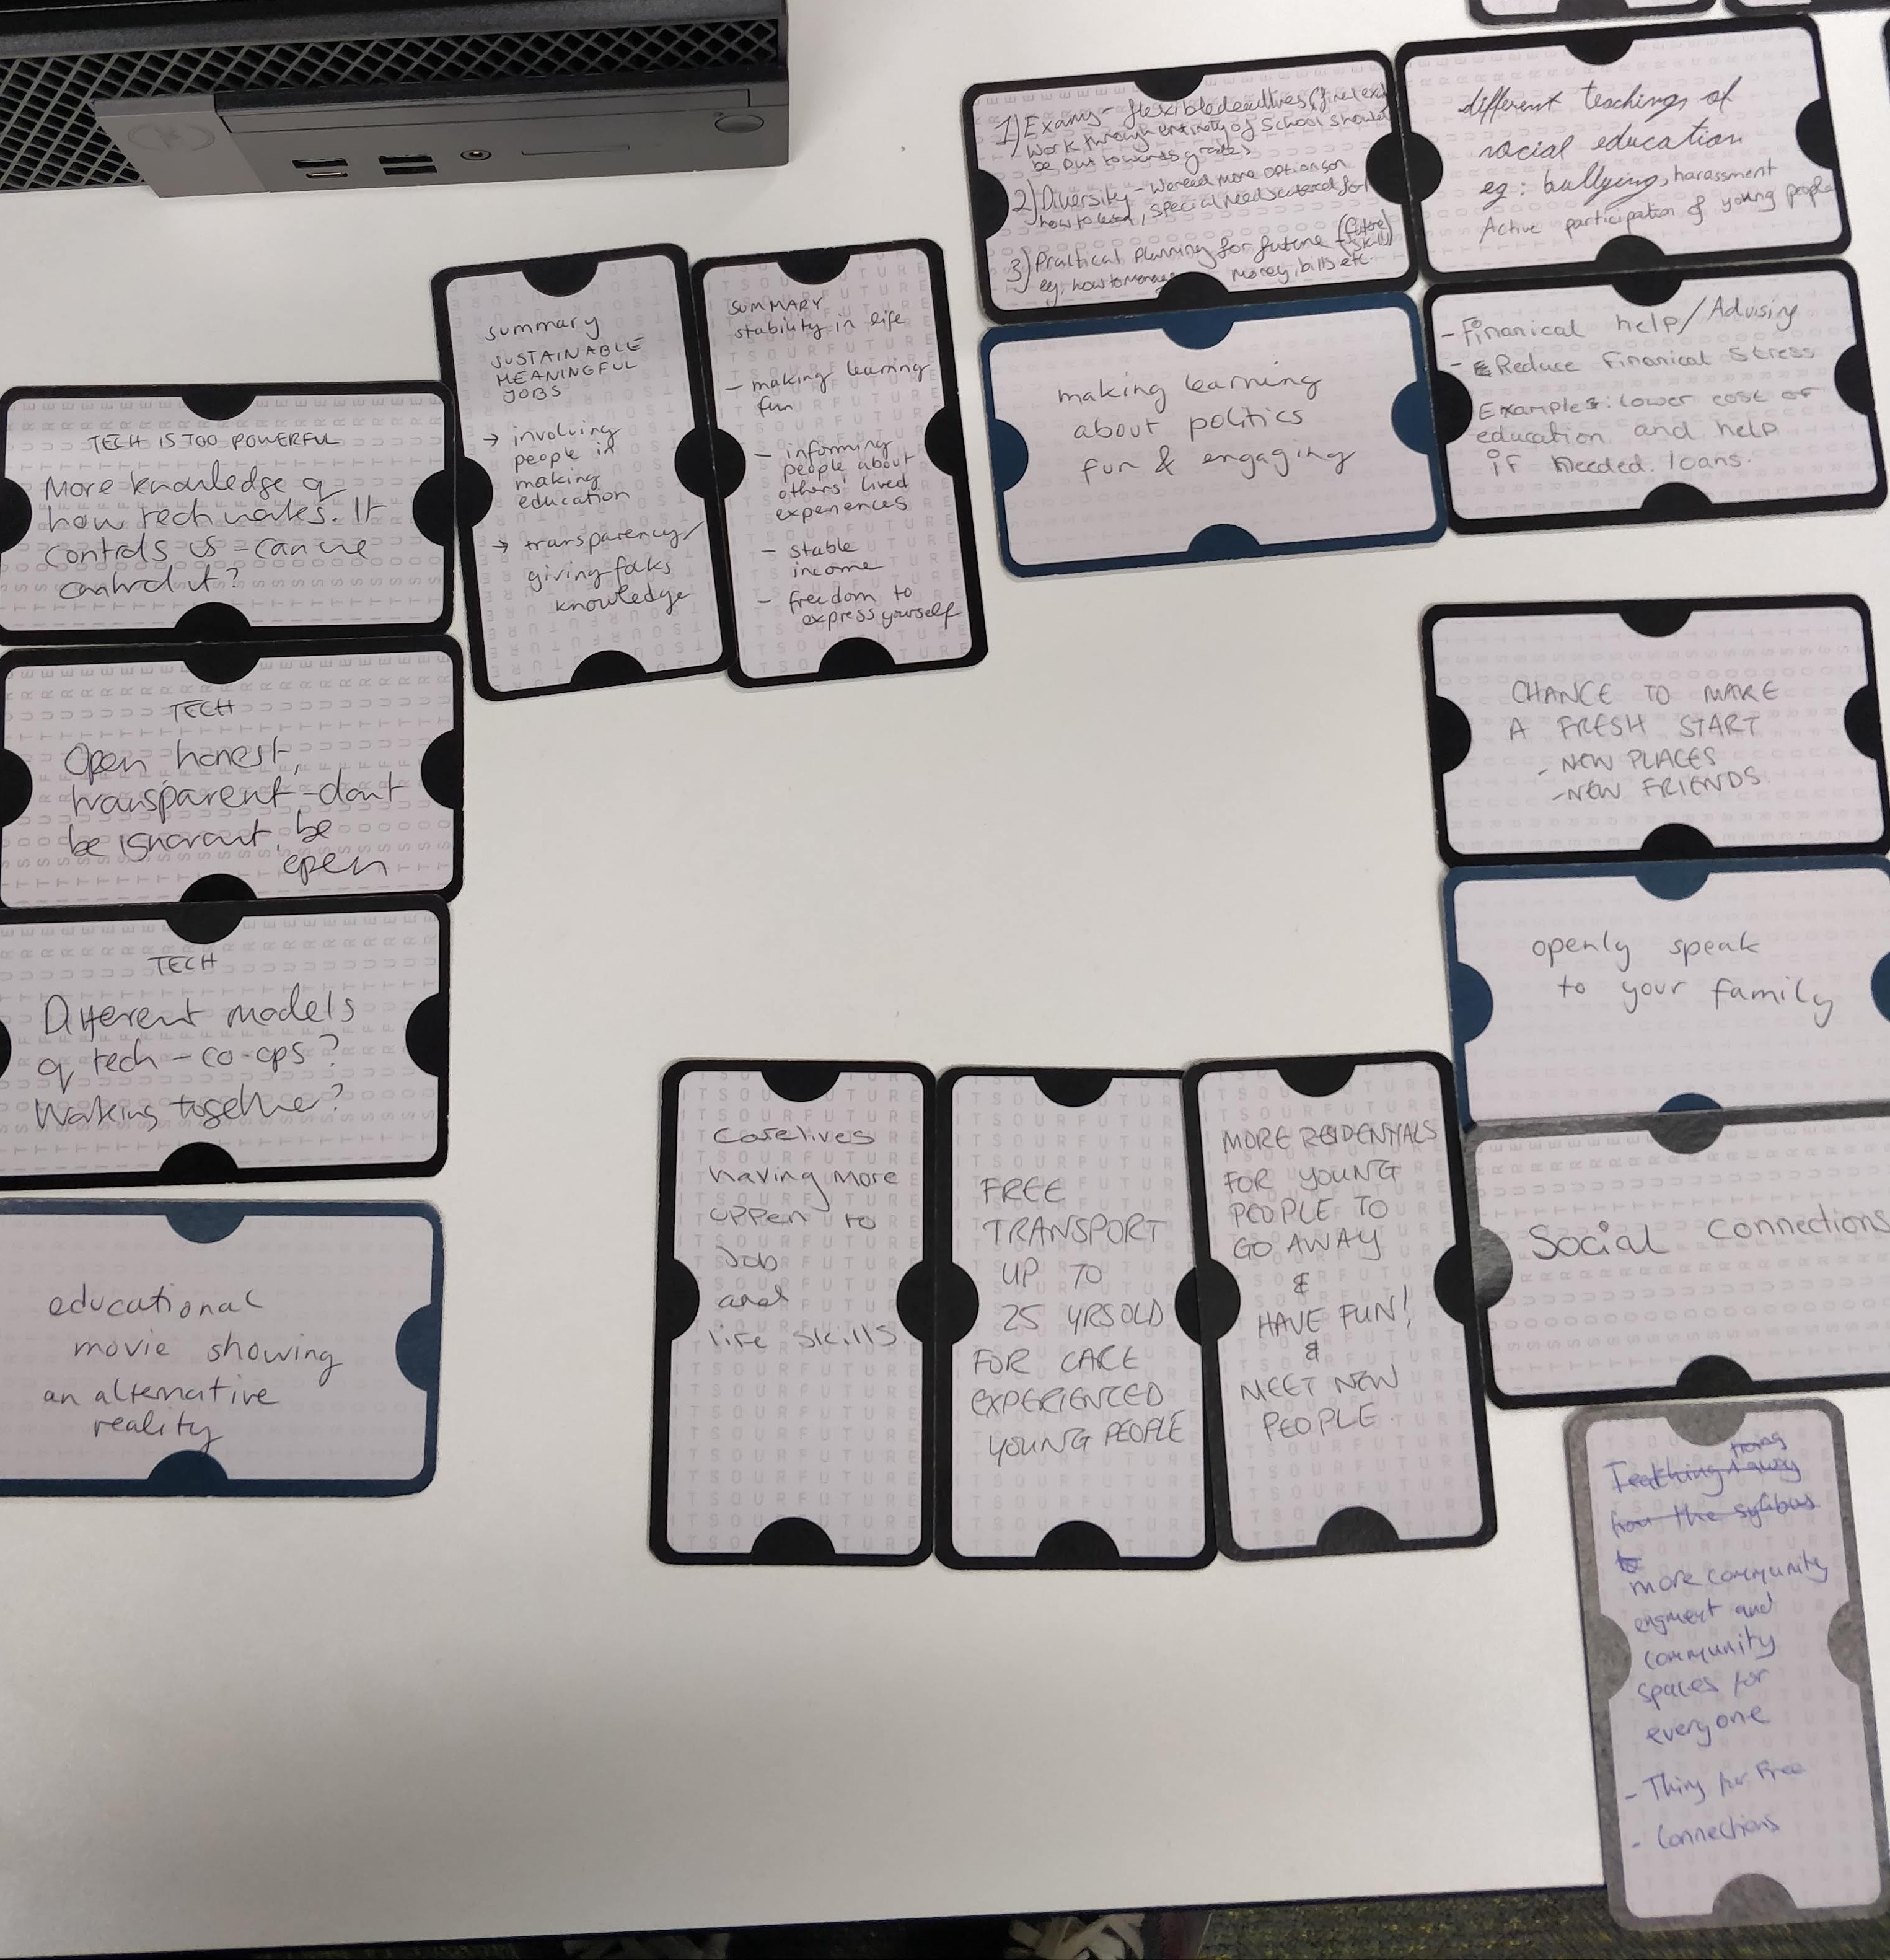
\includegraphics[width=1\linewidth]{Images/7/summary-cards-eg.jpg}
    \caption{A selection of summary cards from \textit{It's Our Future}, clustered by theme.}
    \label{fig:summary-cards-eg}
\end{figure}

The ideas created through the event were sufficiently developed to create a manifesto (an excerpt of which is shown in figure \ref{fig:iof-manifesto}, though the view manifesto is available in appendix \ref{appendix:ios-manifesto}) from them. I developed the manifesto in the weeks after the event, developing six key themes from the dataset and using as much of the participants' own language as possible. These themes were:
\begin{itemize}
    \item Let us use our power (involving young people more deeply in public decision-making)
    \item Support our mental health and wellbeing (properly resourcing and supporting mental health support provision),
    \item Education that works for everyone (expanding methods of teaching and access to education),
    \item Building communities and opportunities (making communities safer and more accessible),
    \item Technology that works for us (reclaiming autonomy over tech usage and design), and
    \item Action on climate change now (moving towards the use of renewable energy sources).
    \end{itemize}
\begin{figure}
    \centering
    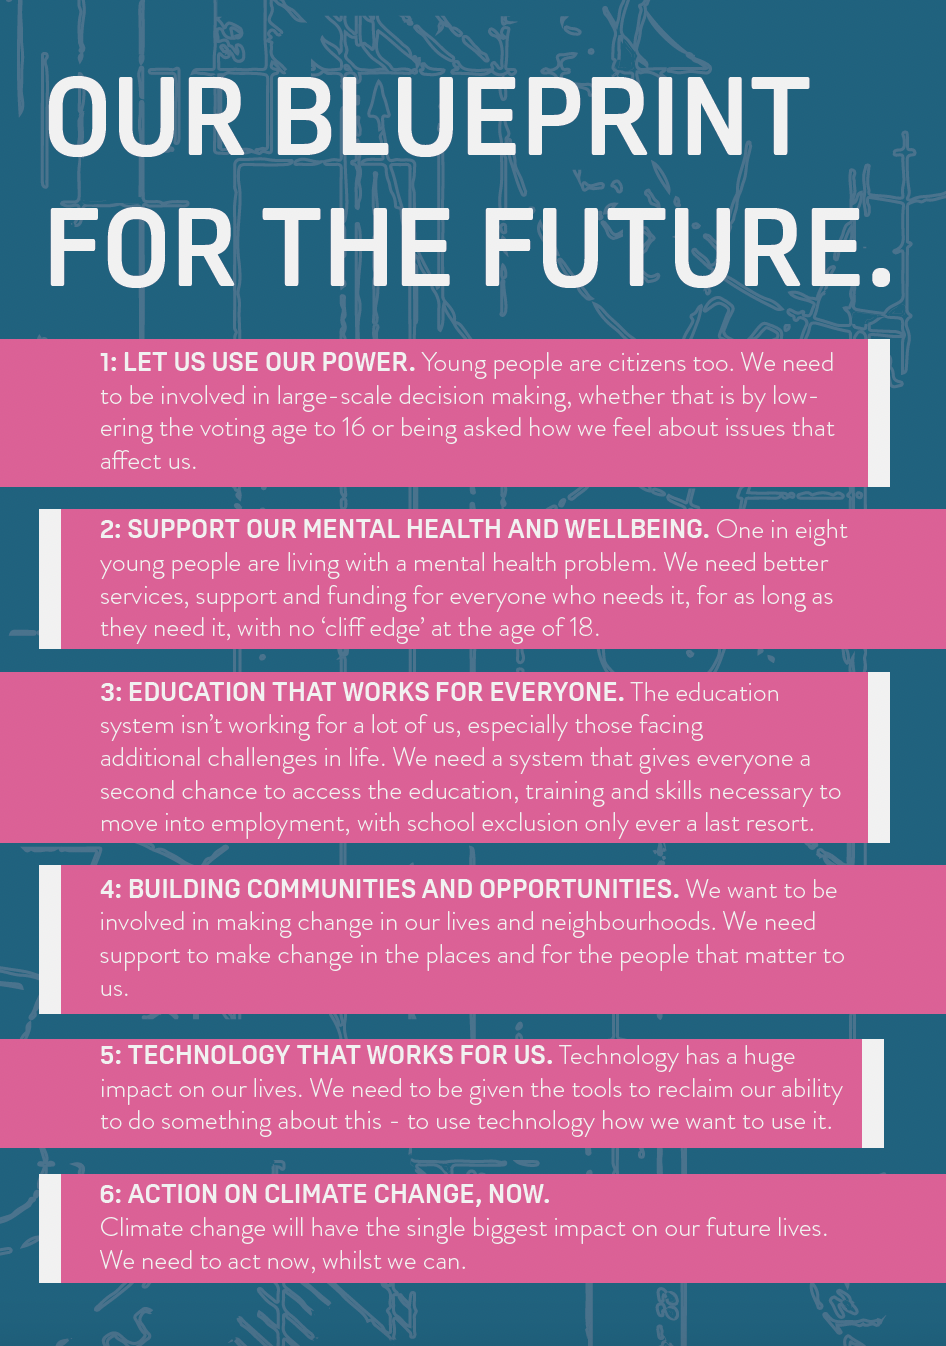
\includegraphics[width=1\linewidth]{Images/7/iof-manifesto.png}
    \caption{A page from the \textit{It's Our Future} manifesto.}
    \label{fig:iof-manifesto}
\end{figure}
Several of the cards from the first activity were issues that were entirely centered on capital - for instance, "job", "my own business", "fame", "winning the lottery", "money", "no debt" and "uni becomes free". In a state of advanced capitalist realism, it is easy to see why these would feel like some of the most transformative changes possible - highlighting the increase in wealth (or stability of wealth) rather than viewing the future in terms of the changes that increased wealth could bring with them. None of the final cards focused simply on capital. The only cards that did speak in terms of any of these areas was significantly more advanced, proposing "sustainable meaningful jobs", suggesting "involving people in making education" and "making learning fun" in order to reach a "stable income". This too has a greater sense of critical consciousness, as instead of conceptualising social change in terms of individual increased capital, the policy proposal instead becomes to change the education system in order to create jobs that can employ people more meaningfully in things that they are interested in and provide them with a more stable income. The most radical suggestion of any of these proposals suggested "making money just for luxuries", with everything else (such as food, clothing, and housing) provided for by taxation. The \textit{It's Our Future} methods are evidently effective at connecting individual's lived experiences to a wider collective and supporting people to build critical consciousness/idea counterpower. 

\subsection{A greater emphasis on skills, resources, and the future}
Although \textit{It's Our Future} did support its participants to consider the kinds of changes that they might want made, it was relatively unsuccessful in bringing about those changes. In part, this was due to a breakdown in our relationship with The Charity, Martin's exit from the team, and the recently-announced General Election becoming a greater priority for them. Yet this was also partly due to the setup of the event and the methods themselves. The first activity was good at getting participants to make connections between individual experiences and the need for wider societal changes - but the later activities gave little sense of how these changes might come about. One of the project's aims had been to help young people build physical counterpower through the exchange of skills and resources. Although this would have been unlikely to happen at the event itself, the event could have created relationships between people that facilitated this exchange of skills and resources after it. As far as I am aware, this did not happen. There was no aspect of the activities that substantively engaged with questioning how these kinds of changes get made, what skills might be useful to support this, and how to map the assets, skills, and resources around people. 

Additionally, although envisioning possible futures was intended to be an integral aspect of the workshop, in practice this activity was fairly limited. Whilst the prompt cards were meant to act as a support to give participants specific scenarios to envision futures for, they may have limited participants' imaginations about what the future could be. For example, in a discussion around what going to a movie with friends would be like if there were better mental health services, participants commented that they would "be less anxious and their friends would be more understanding". Whilst this would have been a significant change in their lives, it perhaps doesn't dig substantively enough into the ways that future would be different and instead just focuses on the state of being able to do something. In a relatively expansive activity, the prompt cards may have re-introduced too much constraint. It would therefore be useful to place a greater emphasis on skills, resources, and imagining alternate futures in the next iteration of these methods. There is a need for a deeper look into which kinds of methods support participants to imagine different kinds of futures that aren't constrained by austerity-intensified capitalist realism. 
\begin{figure}
    \centering
    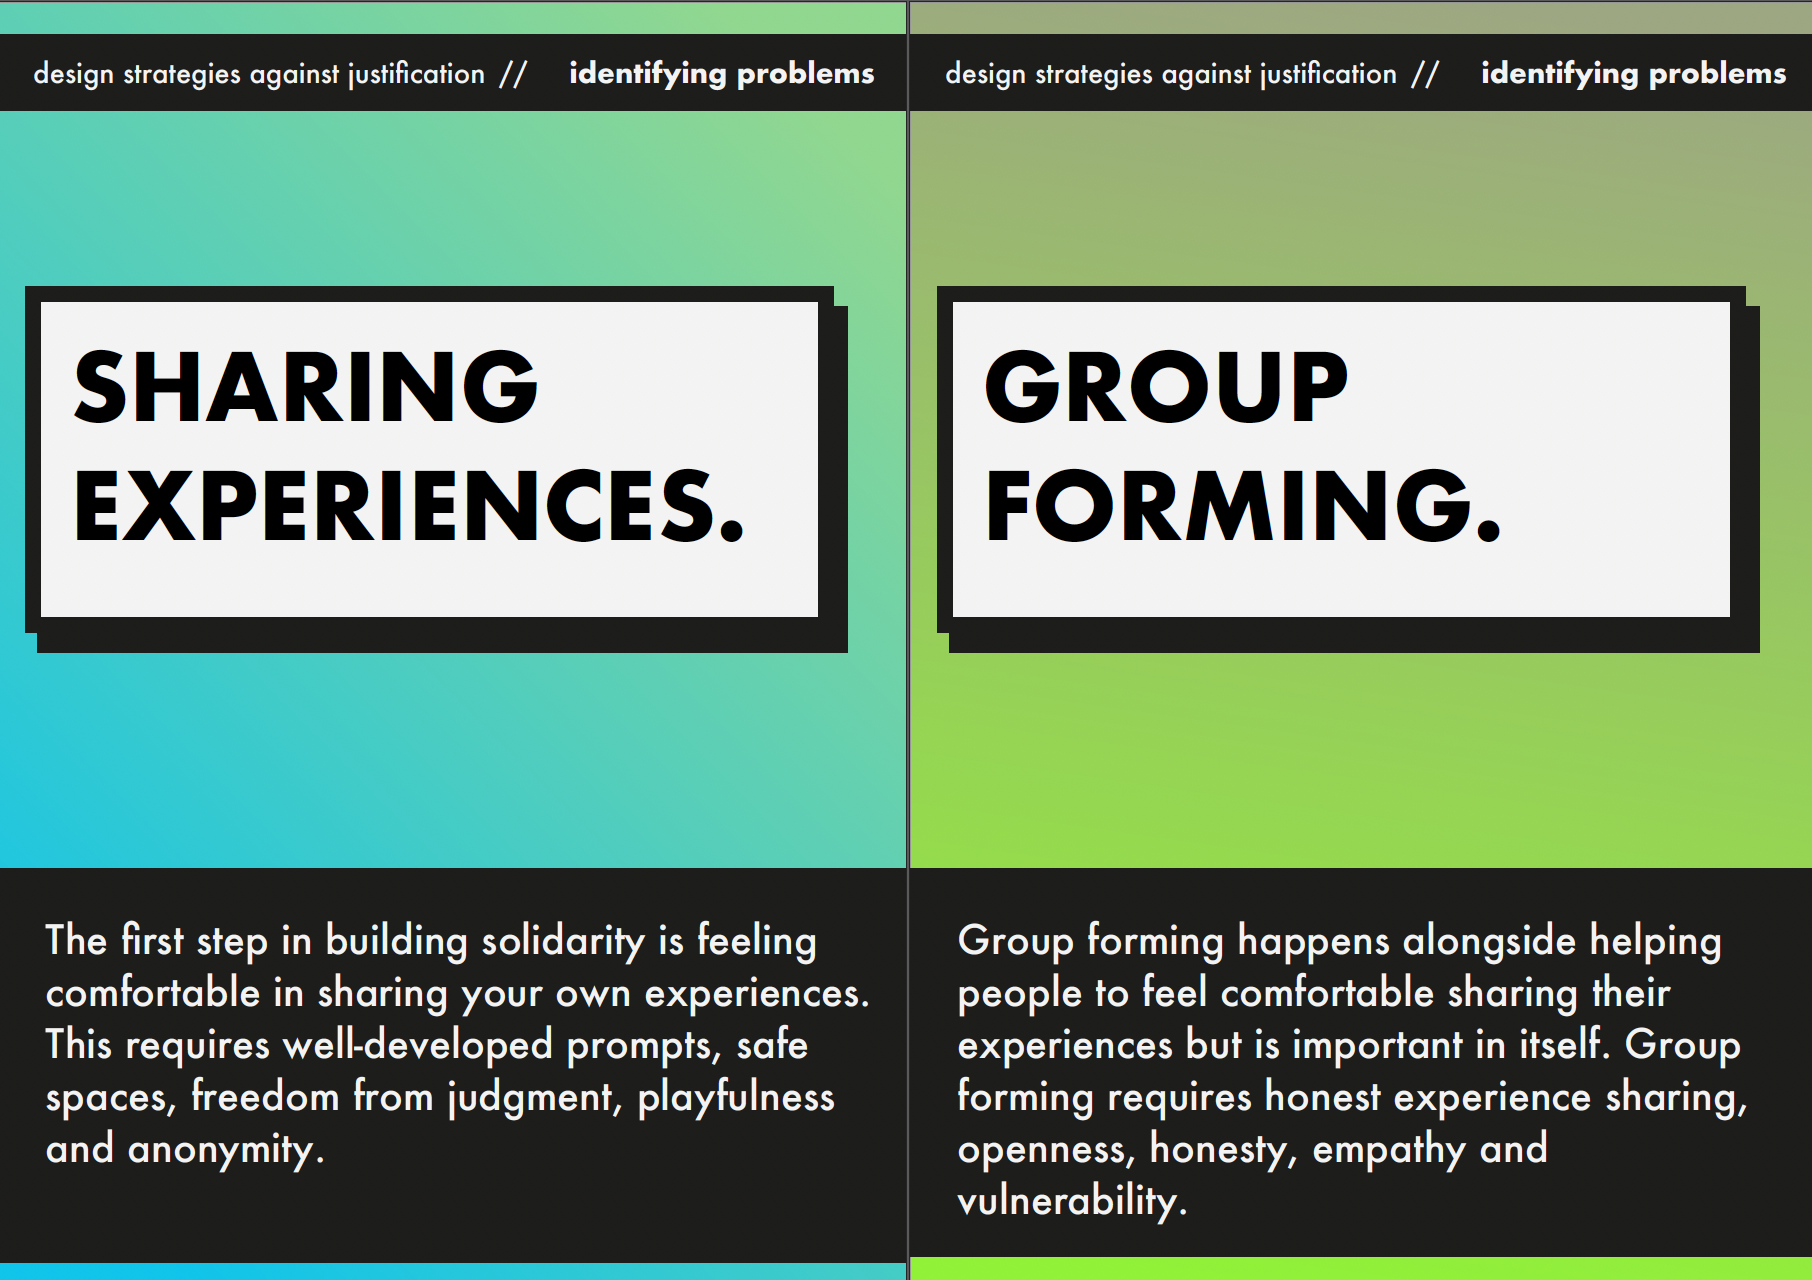
\includegraphics[width=1\linewidth
]{Images/7/design-strats-1.png}
    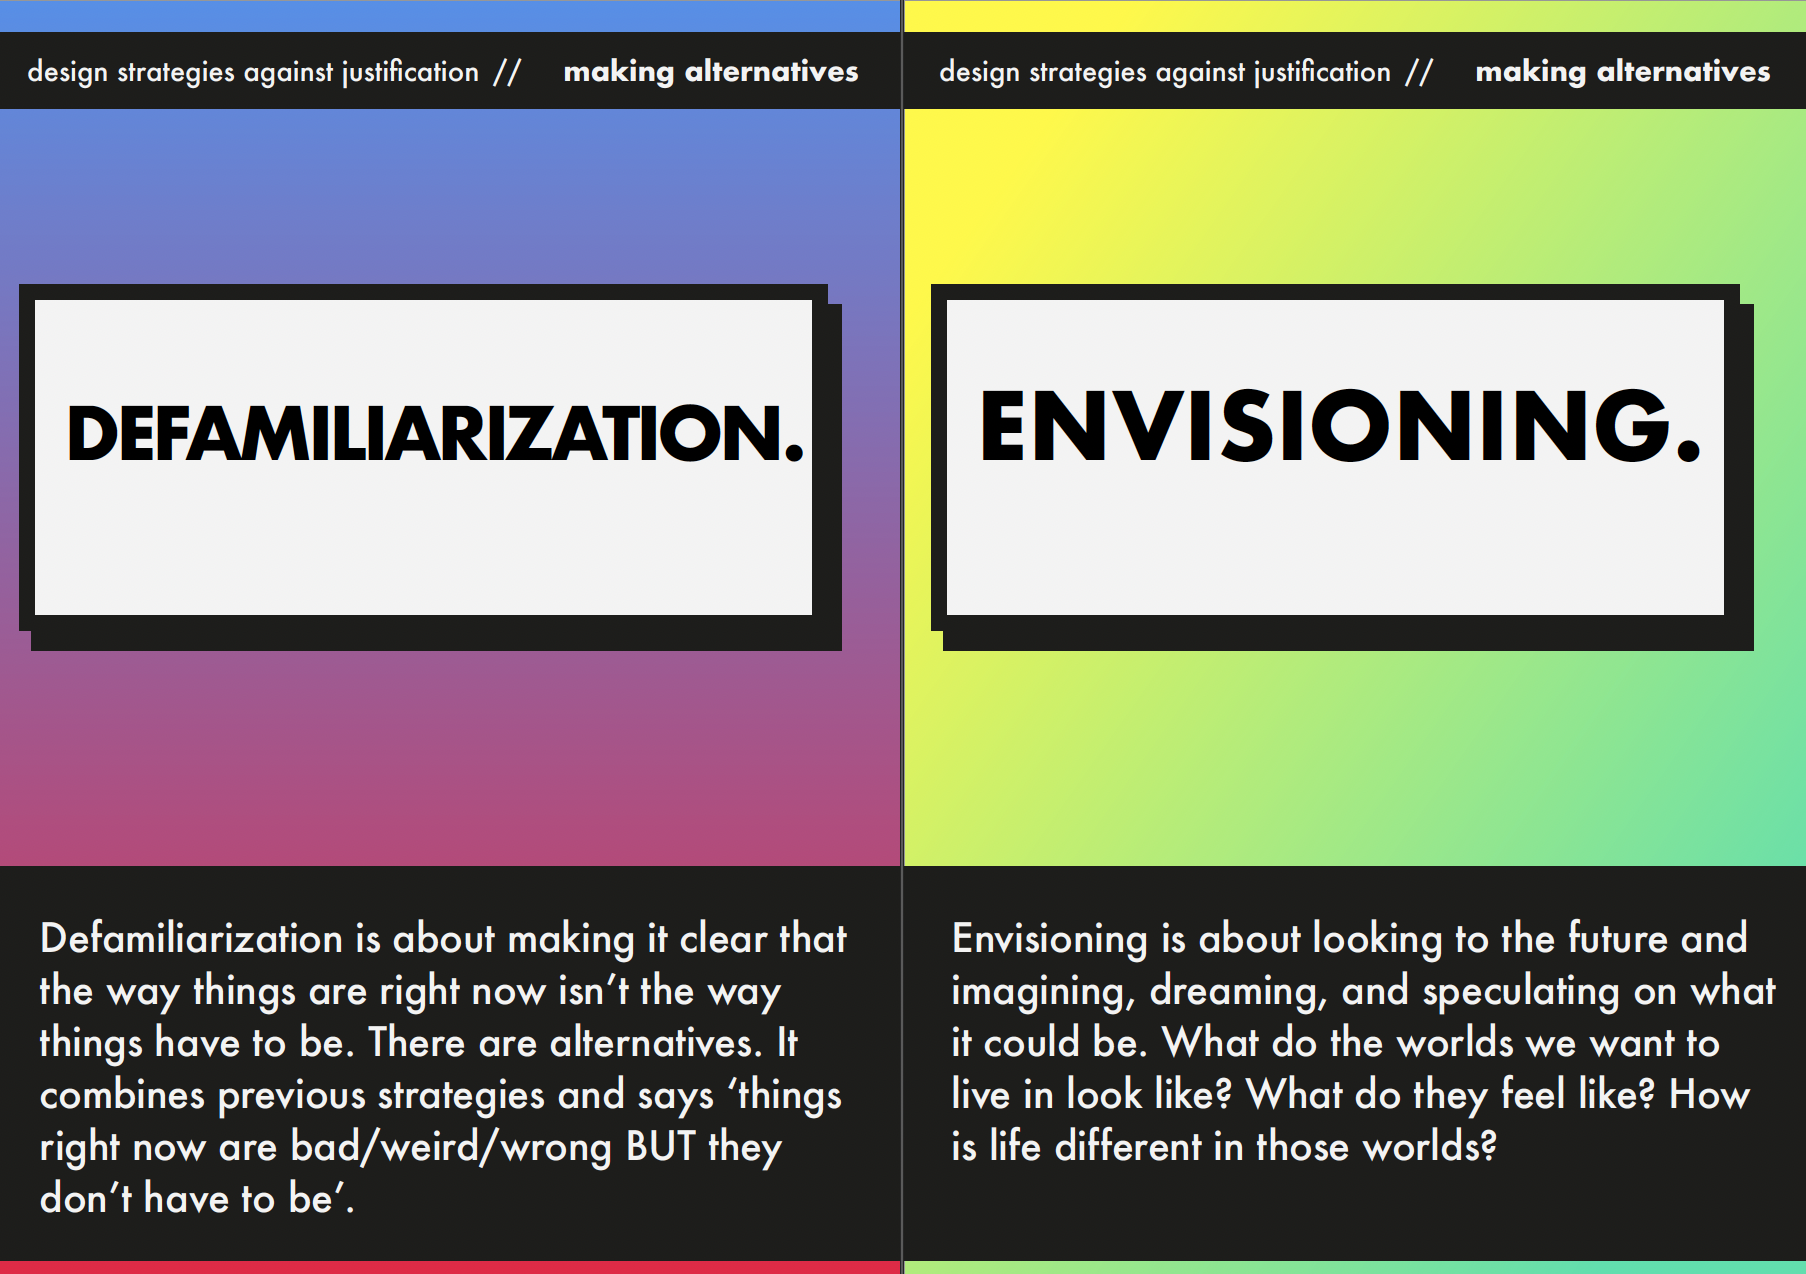
\includegraphics[width=1\linewidth]{Images/7/design-strats-2.png}
    \caption{An excerpt of \textit{Design Strategies against Justification Practices}.}
    \label{fig:design-strats}
\end{figure}
As \textit{It's Our Future} had been a relatively messy project due to the short timeframe, poor communication, and re-presentation of justification practices, I spent some time after the conclusion of \textit{It's Our Future} attempting to identify what each of the methods we had used in the workshop were trying to do and how these might work most effectively. I compiled these in a document called \textit{Design Strategies against Justification Practices} (pictured in figure \ref{fig:design-strats}). I split these methods and approaches into three areas – identifying problems, making alternatives, and principles for doing this work. The principles are "pedagogies", "playfulness", "situated sense-making" and "healing", communicating the general approach we took within the project of thinking about skill exchange, being playful, supporting people to make sense of their own experiences, and where possible, supporting them to heal from them and integrate difficult experiences. The strategies within identifying problems included "sharing experiences", "group forming", "problematising" and "connecting experiences". Broadly, these four strategies were used in the first activity in \textit{It's Our Future}, whereby people shared their own experiences, connected these experiences, formed trust and built a group, and managed to problematise their experiences and link them to wider structural factors. The strategies within making alternatives included "deconstruction", "defamiliarisation", "envisioning" and "building". The second activity of \textit{It's Our Future} used deconstruction and defamiliarisation to unpack the experiences shared in the first activity. As a method, deconstruction breaks something into its constituent components (who was involved? what did they do?) whilst defamiliarisation makes clear that how things are right now are not how they have to be, by making the familiar feel less familiar. The third activity of \textit{It's Our Future} focused on envisoning, and the fourth activity focused on building. Through the lens of \textit{Design Strategies against Justification Practices}, it perhaps becomes a little clearer why there was less on skills, resources, and envisioning futures at the \textit{It's Our Future} event - there were four methods used in the first activity, two in the second, and only one in the third and fourth each. There was a need to develop a more refined approach to these methods. 

\subsection{Failure to avoid justification practices and discursive accumulation}
The initial intention of the \textit{It's Our Future} project was to explore ways to work against the changes made by austerity-intensified capitalist realism in the form of justification, classification, and discursive accumulation practices. Although the project indicates some promising directions to explore, it cannot be said that it had successfully identified the ways that design methods can help mitigate or construct an alternative to the worst of austerity-intensified capitalist realism. This project was plagued by issues of justification and performativity from the outset, and in retrospect would have always struggled. Working this closely with the senior leadership of The Charity meant exposing myself and the project to the clearest version of the forces described in the previous chapter, as indicated by my own experiences becoming more closely aligned with those of my participants. 

The issues did not stop with the change to the in-person workshop format. We continued to have bureaucratic issues during the design process, with further back-and-forth around the exact composition of the activities and structure of the day. At one point I was asked to write a briefing note for the CEO of The Charity, Jason, who attended the event. On the day, he was somewhat of a problem participant. I had given the facilitators strict instructions to prioritise the experiences and viewpoints of young people over those of the "civic leaders" or workers. The facilitator who was running the table that Jason was on had to deal with him continually interrupting the flow of the session to quiz young people in more detail about their experiences. The facilitator reported back to me that "it became very personal, rather than looking at the issues from the top down. He also reacted in a slightly ‘sad’ way, which kind of goes against the vibe of ‘we can change this!’". He repeatedly re-directed conversation in an attempt to extract the most information from young people about their lives. After the event, he emailed the project team saying:
\blockquote{Listening to their lived experience reminded me yet again of how shallow my knowledge is of the challenges they face, day in day out. I really wished that some senior ministers could have been there to listen too.
I think it was a very powerful learning experience for us all, and now we must do our best to turn what we heard into key messages that we can share far and wide.}
The presence of Jason at the event risked perpetuating the exact dynamics that it stood against, as he sought to classify young people as vulnerable, listen to them extractively, and prioritise discursive action over material action. Additionally, The Charity had paid for a videographer to film the event. This meant that throughout the workshop, we had to contend with videographers taking participants out of their groups for interviews to camera and staged B-Roll. This is a clear example of The Charity's drive towards discursive accumulation, as they focused on the production of a visual artefact about the day at the potential cost of making material change at the workshop itself. This continued into the narrative of the video itself, as The Charity attempted to position themselves as benevolent listeners who were capable of solving young people's problems. In the video, Jason reflects on his experience of the day:

\blockquote{I've been shaken by many of the things that young people have talked about - their lived experience of how complex their lives are, how broken the support systems are, and how unsupported they feel - and how difficult their existence was before they came into touch with The Charity.}

The Charity continued to prioritise themselves and their image in the aftermath of the project. We had been preparing the manifesto and event analysis, and had agreed that we would co-develop a plan of follow-up engagement after the project. During the planning process of the event, a General Election was called, and The Charity were keen to use the manifesto as a means to influence candidates to support pledges that would benefit young people's lives. Towards the end of the manifesto creation process, we went back and forth with senior members of The Charity’s team to fight over individual word choices. Linda (Jason's chief of staff) repeatedly tried to convince me to misrepresent the research we had conducted by changing young people's language in order to be more "politically savvy". Linda repeatedly assured me that this "wasn't an optics thing", or "an agenda-driven thing", but that it was more about "an impression". Linda suggested that the people that we wanted to make changes as a result of this document expected to see certain kinds of words, and that it was important to "translate" what we heard into that language. Whilst we managed to resist their changes, our working relationship was soon to be over; we shared a draft version of the manifesto with them, and then they shared it online without ever notifying us, and began their own programme of engagement without us. The Charity were keen to be the face of trying to make change for young people's futures, continuing to manage their reputation and image above all else. 

\section{Conclusion}
In this chapter, I outlined a set of principles and goals for a successful design response to resist austerity-intensified capitalist realism. I explored the different kinds of intervention that could be developed in order to resist justification, classification, and discursive accumulation practices with both young people perceived to be vulnerable and frontline workers. I then described the \textit{It's Our Future} project, its initial form as a "digital conversation", and the research and design work that I did with a small team to identify methods of movement-building and ways to infrastructure participation across multiple forms of social media. I detailed the way that justification practices re-presented themselves throughout the project, eventually culminating in The Charity asking us to take on bureaucratic and legal responsibility for the project. I then detailed the change to an in-person large-scale workshop focused on developing critical consciousness, imagining possible futures, and identifying ways to work towards these.

This chapter began to address my third research question, "How can the tools and methods of design be used to respond to the challenges presented by capitalist realism?", and identified some promising initial directions in the form of methods that are centered on the identification of problems and creating alternatives. The methods used in the \textit{It's Our Future}o project were relatively successful at getting participants to develop critical consciousness of the wider issues around the problems they experienced in their individiual lives. Despite this, they were relatively unsuccessful in meeting the overall aims of mitigating, resisting, or making an alternative to the harms brought about by austerity-intensified capitalist realism. In the next chapter, I detail \textit{fractured signals}, a project which develops on the methods presented in this chapter, and present speculative praxis as a way to mitigate, resist, and create alternatives to austerity-intensified capitalist realism. 